\documentclass[% -- opções da classe memoir --
	12pt,				% tamanho da fonte
	%openright,			% capítulos começam em pág ímpar (insere página vazia caso preciso)
	%twoside,			% para impressão em verso e anverso. Oposto a oneside
	a4paper,			% tamanho do papel. 
	english,			% idioma adicional para hifenização
	brazil				% o último idioma é o principal do documento
	]{abntex2}

%##############################################################%
%                     INCLUSÃO DOS PACOTES                     %
%%%%%%%%%%%%%%%%%%%%%%%%%%%%%%%%%%%%%%%%%%%%%%%%%%%%%%%%%%%%%%%%
% Definindo teoremas e similares. Contador unico, vinculado a capítulos.

\newtheorem{theorem}{Teorema}[chapter]% contador vinculado a capitulos
\newtheorem{corollary}[theorem]{Corolário}
\newtheorem{lemma}[theorem]{Lema}
\newtheorem{proposition}[theorem]{Proposição}
\newtheorem{axiom}[theorem]{Axioma}
%\theoremstyle{definition}
\newtheorem{definition}[theorem]{Definição}
\newtheorem{example}[theorem]{Exemplo}
%\theoremstyle{remark}
\newtheorem{remark}[theorem]{Observação}
%###############################################################%

%%%%%%%%%%%%%%%%%%%%%%%%%

\usepackage[pdftex]{graphics}
\usepackage{epstopdf}
\usepackage{graphicx}
\usepackage{adjustbox}
\usepackage[tableposition=top]{caption}
\newcommand{\source}[1]{\caption*{Fonte: {#1}}}
\usepackage{svg}
\usepackage{rotating}
\usepackage[utf8]{inputenc}
\usepackage[paper=portrait,pagesize]{typearea}

%%%%%%%%%%%%%%%%%%%%%%%%%%%%%

\usepackage[T1]{fontenc}
\usepackage[brazil]{babel}
%\usepackage[dvips]{graphicx}
\usepackage{geometry}
\usepackage{times}
\usepackage{indentfirst}
\usepackage{type 1cm}
\usepackage{lettrine}
\usepackage{colordvi}
\usepackage{colortbl}
\usepackage{multirow}
\usepackage{pstricks}
\usepackage{pstricks-add}
\usepackage{array}

\usepackage{yfonts}
\usepackage{epsf}
\usepackage{wrapfig}
\usepackage{xtab}
\usepackage{eucal}
\usepackage{mathrsfs}
\usepackage{amsmath}
\usepackage{cleveref}
\usepackage{footmisc}
\usepackage{ifthen}

%Extra
\usepackage{algorithmic}
\usepackage[portuguese,portuguesekw,ruled,lined]{algorithm2e}

%Extra
%\usepackage{calligra}          % Fonte caligr\'{a}fica
%\usepackage{suetterl}          % Fonte caligr\'{a}fica
\usepackage[utopia]{quotchap}   % Formata\c{c}\~{a}o para cap\'{\i}tulos
\usepackage{IEEEtrantools_mod}
\usepackage{lscape}


\usepackage[notintoc,portuguese]{nomencl}
\makenomenclature
\usepackage{lastpage}
\usepackage{setspace}
\pagestyle{plain}
\usepackage{cite}
\usepackage{color}
\usepackage{amssymb}
\usepackage{hyphenat}

%%%%%%%%%%%%% Margens %%%%%%%%%%%%

\geometry{a4paper,left=3cm,right=2cm,top=3cm,bottom=2cm}
%\setlength{\beforechapskip}{20pt}

%%%%%%%%%%%%% Outras %%%%%%%%%%%%

%\hypersetup{backref,%
%            pdfpagemode=FullScreen,%
            %colorlinks=true,%
            %citecolor=orange,%
            %urlcolor=blue, %
           % pdfauthor={}, %
            %pdftitle={Redes Ópticas}, %
           % pdfcreator={}, %
            %breaklinks=true, %
            %linktocpage=true
            %}%

%\geometry{hmargin={3cm,2cm},vmargin={3cm,2cm}}

%\topmargin = 1.25cm
%\setlength{\hoffset}{-1in}
%\setlength{\voffset}{0in}
%\topmargin = 1.24cm
%\headheight = 0.5cm
%\headsep = 0.7cm
%\voffset = -1in
%\setlength{\topmargin}{1cm}
%\setlength{\headheight}{0.5cm}
%\setlength{\headsep}{1.5cm}
%\setlength{\marginparsep}{0pt}
%\setlength{\marginparwidth}{0pt}
%\addtolength{\hoffset}{3cm}




\begin{document}

%Numbered environment
%\newcounter{example}[section]
%\newenvironment{example}[1][]{\refstepcounter{example}\par\medskip
%\noindent \textbf{Example~\theexample. #1} \rmfamily}{\medskip}

%Numbered environment defined with Newtheorem
\newtheorem{SampleEnv}{Sample Environment}[section]
%

%%%%%%%%%%%%%%%%%%%%%%%%%%%%%%%%%%%%%%%%%%%%%%%%%%%%%%%%%%%%%%%%%
%                     INCLUSÃO DOS ARQUIVOS                     %
%%%%%%%%%%%%%%%%%%%%%%%%%%%%%%%%%%%%%%%%%%%%%%%%%%%%%%%%%%%%%%%%%

%%%%%%%%%%%%%%%%%%%%%%%%%%%%%%%%%%%%%%%%%%%%%%%%%%%%%%%%%%%%%%%%%
%              INCLUSÃO DOS ELEMENTOS PRÉ-TEXTUAIS              %
%%%%%%%%%%%%%%%%%%%%%%%%%%%%%%%%%%%%%%%%%%%%%%%%%%%%%%%%%%%%%%%%%

    \begin{center}
%==(CABE?ALHO)========================================================


\includegraphics[height=30mm]{Figuras/Capa/brasao_upe}\\

% \begin{minipage}[b]{0.15\linewidth}
% 
\includegraphics[width=\textwidth]{Figuras/Capa/logo_ppges.eps}
% \end{minipage} \hfill
% \begin{minipage}[b]{0.15\linewidth}
% 
\includegraphics[width=\textwidth]{Figuras/Capa/brasao_upe.eps}
% \end{minipage} \hfill
% \begin{minipage}[b]{0.15\linewidth}
% 
\includegraphics[width=\textwidth]{Figuras/Capa/upelogo.eps}
% \end{minipage}



%
\includegraphics[height=45mm]{Figuras/Capa/brasao_poli.eps}

{\textbf{Universidade de Pernambuco (UPE)}} %\\ \vspace{1ex}

{\textbf{Escola Politécnica de Pernambuco (POLI)}} %\\ \vspace{1ex}

{\textbf{Instituto de Ciências Biológicas (ICB)}} \\ \vspace{1ex}

{\textbf{Programa de Pós-Graduação em Engenharia de Sistemas}} \\ \vspace{1ex}
%=====================================================================

\vspace{1.0in}

{\Large Hugo Abreu Mendes}

\vspace{1.3in}

%===(T?TULO DA DISSERTA??O)================================
{\Large \textbf{MODELOS HÍBRIDOS AUTOMATIZADOS PARA PREVISÃO DE IRRADIAÇÃO E PRODUÇÃO FOTOVOLTAICA}} \\
%=====================================================================

\vspace{1.4in}

{\large Dissertação de Mestrado}


\vspace{1.6in}


\vspace{18pt}{Recife, Março de 2021.}

\end{center}
    %%%%%%%%%%%%%%%%%%%%%%%%%%%%%%%%%%%%%%%%%%%%%%%%%%%%%%%%%%%%%%%%%%%%%%
% CAPA DO PROJETO DE DISSERTA??O
%%%%%%%%%%%%%%%%%%%%%%%%%%%%%%%%%%%%%%%%%%%%%%%%%%%%%%%%%%%%%%%%%%%%%%

\thispagestyle{empty}

\begin{center}

\begin{minipage}[b]{0.15\linewidth}

\includegraphics[width=\textwidth]{Figuras/Capa/logo_ppges.eps}
\end{minipage} \hfill
\begin{minipage}[b]{0.15\linewidth}

\includegraphics[width=\textwidth]{Figuras/Capa/brasao_upe.eps}
\end{minipage} \hfill
\begin{minipage}[b]{0.15\linewidth}

\includegraphics[width=\textwidth]{Figuras/Capa/upelogo.eps}
\end{minipage}

%==(CABE?ALHO)========================================================
{\textbf{Universidade de Pernambuco (UPE)}}% \\ \vspace{1ex}

{\textbf{Escola Politécnica de Pernambuco (POLI)}}%\\ \vspace{1ex}

{\textbf{Instituto de Ciências Biológicas (ICB)}} \\ \vspace{2ex}

{\textbf{Programa de Pós-Graduação em Engenharia de Sistemas}} \\ \vspace{1ex}
%=====================================================================

\vspace{0.8in}

{\Large Hugo Abreu Mendes}\\

\vspace{1in}

%===(T?TULO DO PROJETO DE DISSERTA??O)================================
{\Large \textbf{MODELOS HÍBRIDOS AUTOMATIZADOS PARA PREVISÃO DE IRRADIAÇÃO SOLAR}} \\
%=====================================================================

\vspace{0.3in}

%===(NOME DO ALUNO E DO ORIENTADOR)===================================

%\vspace{1ex} {\textbf{Orientador: Prof$^{a}$. Dr$^{a}$. Maria de Lourdes Melo Guedes Alcoforado} }

%=====================================================================

\end{center}

%===(IDENTIFICADOR DO DOCUMENTO)===================================
\begin{flushright}
    \vspace{0.5in}
    \parbox{3.50in}
    %{\textbf{Dissertação} apresentada à Universidade de Pernambuco como parte dos %requisitos para a obtenção do título de Mestre em Engenharia de Sistemas.
    %\\ 
    %\\Área de concentração: \textbf{Telemática} 
    %}
    {\textbf{Projeto de Mestrado} redigido para o Programa de Pós-Graduação em Engenharia de Sistemas, como parte dos requisitos para defesa de dissertação.
    }

\end{flushright}
%===================================================================

\vspace{1.2ex}

\begin{center}

%===(IDENTIFICA??O DA BANCA DE QUALIFICA??O E DATA(M?S/ANO))========


\vspace{1ex} {\textbf{Orientadora: Prof. Dr. Manoel Henrique da Nóbrega Marinho} }\\
\vspace{1ex} {\textbf{Coorientador: Prof. Dr. João Fausto Lorenzato de Oliveira} }


\vspace{0.2in}
\vspace{18pt}{Recife, Março de 2021.}
%==================================================================

\end{center}


    
%%%%%%%%%%%%%%%% Agradecimentos %%%%%%%%%%%%%%%%%%%%%%%%%%%%%%%%%    
% Pronto, mas para qualificação não precisa
%\chapter*{Agradecimentos}

Agradeço primeiramente aos professores do Programa de Pós Graduação em Engenharia de Sistemas da POLI, por não se esforçados para manter o compromisso com os discentes e oferta de disciplinas em um ano tão difícil como o de 2020. O contexto da Pandemia realmente dificultou muitas coisas, porém com a ajuda do meu orientador Manoel Marinho e do meu coorientador Fausto Lorenzato o trabalho pode ter continuidade com sucesso. No mais agradeço a meus pais pelo suporte.
%
    
    \chapter*{Resumo}

A estimativa de variáveis físicas pode ser feita através de modelagens numéricas variadas. Uma das formas úteis se dá pela analise e modelagem de séries temporais. Dentro do contexto da geração de energias limpas, são feitas previsões de radiação solar, para usinas fotovoltaicas e velocidade do vento para usinas eólicas. Modelos lineares de séries temporais como ARIMA são muito utilizados, porém muito se avançou utilizando técnicas de \textit{machine learning} para melhorar os resultados, que podem ser utilizadas em conjunto com modelos lineares, resultando em modelos híbridos. Neste trabalho é apresentada uma nova forma de automatizar a modelagem SARIMAX a partir do uso em conjunto dos algoritmos de otimização PSO e ACO, levando em consideração a sazonalidade e possíveis variáveis exógenas disponíveis. Também são apresentados 2 modelos híbridas distintos que possuem MLPs como elementos principais. Um protocolo foi utilizado para obtenção dos resultados, que foram obtidos para tais modelos que se mostraram muito promissores para utilização em sistemas automáticos de previsão de radiação.


\noindent\par\vspace{1em}
\noindent\textbf{Palavras-chave: Radiação solar, séries temporais, aprendizado de máquina, otimização} 

%%%%%%%%%%%%% abstract %%%%%%%%%%%%    
% Está pronto, mas Para qualificação não precisa
%\chapter*{Abstract}


\noindent\par\vspace{1em}
\noindent\textbf{Keywords: image transmission, 2-BAC, turbo codes, iterative decoding}
%%%%%%%%%%%%%%%%%%%%%%%%%%%%%%%%%%%
    
    \chapter*{Lista de Abreviações e Siglas}
\linespread{1.5}

ACF - \textit{Auto Correlation Function}\bigskip

ACO - \textit{Ant-Colony Optimization}\bigskip

AG - Algoritmo Genético\bigskip

AIC - \textit{Akaike Information Criterion}\bigskip

ARIMA - \textit{Autoregressive Integrated Moving Average}\bigskip

ARMA - \textit{Autoregressive Moving Average}\bigskip

IID - \textit{Independent,Identically Distributed}\bigskip

LBFGS - \textit{Limited-Memory Broyden–Fletcher–Goldfarb–Shanno Algorithm}\bigskip

ML - \textit{Machine Learning}\bigskip

MLP - \textit{Mult Layer Perceptron}\bigskip

PACF - \textit{Partial Auto Correlation Function}\bigskip

PSO - \textit{Particle Swarm Optimization}\bigskip

RNA - Redes Neurais Artificiais\bigskip

SARIMAX - \textit{Seasonal Autoregressive Integrated Moving Average}\bigskip

SGD - \textit{Stochastic Gradient Descendent}\bigskip




%%%%%%%%%%%%%%%%%%%%%%%%%%%%%%%%%%%%%%%%%%%%%%%%%%%%%%%%%%%%%%%%%
%       LISTAS DE FIGURAS, TABELAS E SUMÁRIO DO TRABALHO        %
%%%%%%%%%%%%%%%%%%%%%%%%%%%%%%%%%%%%%%%%%%%%%%%%%%%%%%%%%%%%%%%%%
     
     % ---
    % inserir lista de ilustrações
    % ---
    \pdfbookmark[0]{\listfigurename}{lof}
    \listoffigures*
    \cleardoublepage
    % ---
    
    % ---
    % inserir lista de tabelas
    % ---
    \pdfbookmark[0]{\listtablename}{lot}
    \listoftables*
    \cleardoublepage
    % ---
    
    % ---
    % inserir o sumario
    % ---
    \pdfbookmark[0]{\contentsname}{toc}
    \tableofcontents*
    \cleardoublepage
    % ---

%%%%%%%%%%%%%%%%%%%%%%%%%%%%%%%%%%%%%%%%%%%%%%%%%%%%%%%%%%%%%%%%%
%          INCLUSÃO DOS CAPÍTULOS (ELEMENTOS  TEXTUAIS)         %
%%%%%%%%%%%%%%%%%%%%%%%%%%%%%%%%%%%%%%%%%%%%%%%%%%%%%%%%%%%%%%%%%

    \chapter{Introdução}
\label{cap:introducao}

\section{Motivação}

Na última década o crescimento da geração fotovoltaica foi expressivo, de acordo com a IEA (Internetional Energy Agency), a produção global saltou de 32TWh em 2010 para mais de 720 TWh em 2020 \cite{ieasolarpvontrack2020}. 

Estimativa de potencial de geração fotovoltaico é um tema que já obteve grande avanço na academia \cite{chin2015cell, jordehi2016parameter, de2017performance}. Os trabalhos levam em consideração a tecnologia utilizada pela célula e modelos de satélite que visam definir os parâmetros físicos de entrada, tais como radiação, temperatura e velocidade do vento \cite{mueller2009cm, huld2012new, amillo2014new, habte2017evaluation}.

A utilização de técnicas de inteligência artificial aplicadas a este tema tem focado na predição temporal de geração \cite{voyant2017machine, wolff2016statistical, li2016hierarchical}. Este tipo de predição é muito útil levando-se em consideração o sistema elétrico completo de uma região ou país, para balanceamento de oferta e demanda, sendo possível uma programabilidade maior para o operador do sistema elétrico, em relação a adequação do uso de outras fontes de energia.

São encontrados alguns métodos de previsão de energia fotovoltaica na literatura, sendo subdivididos de acordo com o horizonte de previsão \cite{mellit2020advanced}. A Tabela \ref{tab:app_forecast} resume os prazos e aplicações para cada método.

\begin{table}[!ht]
\caption{Demonstration of simple table syntax.} 
\label{tab:app_forecast}
\begin{tabular}{c|c|c}
\textbf{Horizonte} & \textbf{Período máximo} & \textbf{Aplicação}                                                                                                               \\ \hline
Curtíssimo prazo   & Minutos                 & \begin{tabular}[c]{@{}c@{}}controle e gestão de sistemas fotovoltaicos\\microredes\\mercado de eletricidade\end{tabular}         \\ \hline
Curto prazo        & 72h                     & \begin{tabular}[c]{@{}c@{}}controle das operações do sistema de potência\\despacho econômico\\comprometimento da unidade\end{tabular} \\ \hline
Médio prazo        & Semanas                  & manutenção e planejamento de usinas fotovoltaicas \\ \hline
Longo prazo        & Anos                     & manutenção e planejamento de usinas fotovoltaicas  \\ \hline                                               
\end{tabular}
\source{Autor.}
\end{table}

Este trabalho busca unir de uma melhor forma o uso da ciência de dados e algoritmos de aprendizado de máquina para estimação de potencial de geração em sítios, levando a otimização da escolha utilizando dados reais de geração e dados de simulação, levando em consideração diversas bases de dados diferentes em um estudo de caso para a região nordeste do Brasil.

\section{Objetivos}

\subsection{Objetivo Geral}

Criar modelos de auto ML capazes de se adaptar e fazer a previsão de séries temporais de irradiação e geração fotovoltaica.

\subsection{Objetivos específicos}

\begin{itemize}
    \item Obter dados atuais de irradiação solar por um período significativo
    \item Obter dados de variáveis exógenas naturais por um período significativo
    \item Obter dados atuais de usinas fotovoltaicas por um período significativo
    \item Corrigir dados obtidos
    \item Gerar modelo linear SARIMAX com os dados obtidos
    \item Treinar modelos híbridos propostos
    \item Avaliar modelos híbridos propostos
    \item Compilar programa de computador para aplicação dos modelos propostos
\end{itemize}

\section{Estado-da-arte}

Modelos híbridos, em que se utiliza da modelagem linear dada por um ARIMA ou variante já foi muito utilizada e discutida na literatura \cite{zhang2003time, khashei2010artificial, babu2014moving, de2014hybrid, de2016hybrid, domingos2019intelligent}.

\section{Estrutura da dissertação}

A organização das seções deste trabalho se dá da seguinte forma. Primeiramente será apresentada a teoria por trás da previsão de séries temporais utilizando modelos lineares \ref{cap:series_temp}, no mesmo capítulo será discutido os dados de series temporais horárias obtidos a partir da base de dados do INMET \cite{INMET}. Em seguida no capítulo \ref{cap:auto_ml} são apresentados os modelos híbridos que utilizam dos algoritmos de machine learning apresentados no capítulo antecedente.
	\chapter{Objetivos}
\label{cap:objetivos}

\subsection{Objetivo Geral}

Criar modelos de auto ML capazes de se adaptar e fazer a previsão de séries temporais de irradiação e geração fotovoltaica.

\subsection{Objetivos específicos}

\begin{itemize}
    \item Obter dados atuais de irradiação solar por um período significativo
    \item Obter dados de variáveis exógenas naturais por um período significativo
    \item Obter dados atuais de usinas fotovoltaicas por um período significativo
    \item Corrigir dados obtidos
    \item Gerar modelo linear SARIMAX com os dados obtidos
    \item Treinar modelos híbridos propostos
    \item Avaliar modelos híbridos propostos
    \item Melhorar modelos híbridos propostos
    \item Compilar programa de computador para aplicação dos modelos propostos
\end{itemize}
    \chapter{Estado da arte}
\label{cap:estado_da_arte}

Modelos híbridos, em que se utiliza da modelagem linear dada por um ARIMA ou variante já foi muito utilizada e discutida na literatura \cite{zhang2003time, khashei2010artificial, babu2014moving, de2014hybrid, de2016hybrid, domingos2019intelligent}. O intuito destes modelos, chamados híbridos, é de que incrementar a capacidade de adaptação da modelagem linear ARIMA for meio de outros algoritmos de \textit{machine learning} ou \textit{extreme learning machines} \cite{yu2020hybrid}, a combinação de modelos pode ser eficaz em aprimorar o desempenho de previsão \cite{khashei2012new}.

Nos últimos anos, foi comum a implementação de modelos de série temporal linear combinado com \textit{machine learning} para previsões de séries temporais, utilizando ARIMA com RNA \cite{xiong2017hybrid}, SVM \cite{domingos2019intelligent}, LSTM \cite{choi2018stock}. Outros modelagens híbridas podem ser feitas, como \textit{Exponential Smoothing} em conjunto com LSTM \cite{smyl2020hybrid}.

Se é muito utilizado algoritmos de inteligência de enxame no processo de otimização de modelos híbridos. Sendo vistos diversas aplicações utilizando os modelos que são abordados nesse trabalho: Algoritmo Genético (GA) \cite{huang2012hybrid}, algoritmo de Otimização de Enxame de Partículas (PSO) \cite{bagheri2014financial, pradeepkumar2017forecasting}, e algoritmo Ant Colony Optimization (ACO) \cite{shen2013optimal}. Mais especificamente sobre previsão de geração fotovoltaica e irradiação solar, o padrão de utilização de modelos se mantém, \cite{sobri2018solar, wang2019review}, havendo um destaque maior para o uso de \textit{deep learning}.

O uso de algoritmos meta-heurístico para implementação de sistemas automatizados (autoML) pode ser dividido em duas vertentes, sendo otimização de hiper-parâmetros e otimização arquitetural \cite{he2021automl}. Neste trabalho, o protocolo proposto para o AutoML consta com as vertentes. Do ponto de vista de implementação, Python é a linguagem mais utilizada em inteligência artificial e \textit{machine learning}, muito devido a facilidade de distribuição de códigos e pacotes, e adoção da comunidade desenvolvedora \cite{blank2020pymoo}. Dentre as bibliotecas mais utilizadas está o \textit{Scikit-Learn}, por conta da sua facilidade de uso, consistência e grande leque de algoritmos disponíveis \cite{scikit-learn, hackeling2017mastering}. 

Além do \textit{Scikit-Learn}, bibliotecas como Keras, que se trata de um envelopamento de auto nível que facilita a construção de redes neurais profundas \cite{jin2019auto} e outros softwares muito utilizados, como WEKA, também constam com camadas de automatização \cite{feurer2020auto}. Neste trabalho, é desenvolvida uma biblioteca específica para series temporais, de acordo com o que é mostrado no capítulo \ref{cap:materiais_e_metodos} sobre materiais e métodos, e também com o protocolo definido na seção \ref{sec:protocolo_resultados}.
    \chapter{Materiais e Métodos}
\label{cap:materiais_e_metodos}

\section{Modelagem de Séries Temporais}
\label{sec:series_temp}

\subsection{Séries temporais}

Series temporais se tratam de um conjunto de observações orientadas no tempo \cite{brockwell2002introduction}. Diferentemente de sinais, series temporais são sempre discretas.

O fato de series temporais serem denominadas dessa forma está na correlação temporal de cada um dos seus pontos. A correlação temporal significa que cada observação pode ser linearmente modelada por observações passadas. 

\subsection{Modelos Lineares}

\subsubsection{ARIMA}

Dada uma série temporal definida como $X_t$ sendo $t$ o índice inteiro de cada observação, o modelo ARMA$(p^{'},q)$ é dado pela Equação \ref{eq:arma_model} abaixo, o parâmetro $\alpha_i$ é responsável pela parte auto regressiva do modelo, enquanto que $\theta_i$ pela média móvel. O termo $\varepsilon_t$ representa o erro que é assumido como uma variável aleatória IID, amostrada a partir de uma distribuição normal com média zero \cite{brockwell2002introduction}. 

\begin{equation}
\label{eq:arma_model}
    X_t-\alpha_1X_{t-1}- \dots -\alpha_{p'}X_{t-p'} = \varepsilon_t + \theta_1 \varepsilon_{t-1} + \cdots +\theta_q \varepsilon_{t-q}
\end{equation}

Uma outra forma de descrever o modelo ARMA é obtida ao se utilizar o operador $L$ que representa os \textit{Lags}, como sendo índices do passado em relação a uma variável, como na Equação \ref{eq:arma_model_L}.

\begin{equation}
\label{eq:arma_model_L}
    \left(1 - \sum_{i=1}^{p'} \alpha_i L^i\right) X_t=\left(1 + \sum_{i=1}^q \theta_i L^i\right) \varepsilon_t
\end{equation}

Assumindo que o polinômio $\left( 1 - \sum_{i=1}^{p'} \alpha_i L^i \right)$ possui uma raiz unitária como um fator de  $(1-L)$ de multiplicidade $d$, então a Equação \ref{eq:arma_model_L} pode ser reescrita como \ref{eq:arma_model_alpta2phi}.

\begin{equation}
\label{eq:arma_model_alpta2phi}
    \left(1 - \sum_{i=1}^{p'} \alpha_i L^i\right)=\left(1 - \sum_{i=1}^{p'-d} \varphi_i L^i\right)\left(1 - L \right)^d
\end{equation}

O modelo ARIMA$(p,d,q)$ é uma derivação do modelo ARMA ao expressar a fatoração polinomial mostrada anteriormente, substituindo \ref{eq:arma_model_alpta2phi} em \ref{eq:arma_model_L} e definindo $p=p^{'} - d$, o que leva a equação \ref{eq:arima_model}.

\begin{equation}
\label{eq:arima_model}
    \left( 1 - \sum_{i=1}^p \varphi_i L^i \right) (1-L)^d X_t = \left( 1 + \sum_{i=1}^q \theta_i L^i \right) \varepsilon_t \
\end{equation}

A equação \ref{eq:arima_model} pode ser ainda simplificada da forma \ref{eq:arima_model_simple}, esta simplificação ajuda a na modelagem SARIMAX que seguirá na próxima seção \ref{subsec:sarimax}.

\begin{equation}
\label{eq:arima_model_simple}
    \phi_p(L)(1-L)^d X_t = c + \theta_q(L)\varepsilon_t
\end{equation}

Em que, $\phi_p(L)$ se torna o termo auto regressivo de ordem $p$, $c$ é uma constante e $\theta_q(L)\varepsilon_t$ o termo de médias móveis de ordem $q$, $d$ é a ordem de diferenciação. 

A teoria dos modelos ARIMA teve sua ampla aplicação por conta dos esforços dos trabalhos de Box et al. \cite{box2011time}, que desenvolveu um método sistemático, iterativo e prático de construção de modelos \cite{ramos2015performance}, dividido em três etapas, identificação do modelo, estimativa de parâmetro e diagnóstico do modelo.

\subsubsection{SARIMAX}
\label{subsec:sarimax}

A partir da equação \ref{eq:arima_model_simple} que descreve um modelo ARIMA não sazonal é possível chegar a modelagem SARIMAX, que leva em conta a sazonalidade e também variáveis exógenas. Primeiramente, o modelo SARIMA, que leva em consideração apenas a sazonalidade é representado pela equação \cite{arunraj2016application, de2018modelo}

\begin{equation}
\label{eq:sarima_model}
    \phi_p(L)\Phi_P(L^S)(1-L)^d(1-L^S)^D X_t = c + \theta_q(L)\Theta_Q(L^S)\varepsilon_t
\end{equation}

Em que, $\Phi_P(L^S)$ se torna o termo auto regressivo sazonal de ordem $P$, $S$ é a frequência de sazonalidade, deve ser 12 para dados mensais e 24 para dados horários. $D$ é a quantidade de diferenciações para a parte sazonal do modelo e $\Theta_Q(L^S)$ se trata do termo de médias móveis sazonal.

O modelo SARIMA tem capacidade de lidar séries temporais estacionárias e não estacionárias com elementos sazonais \cite{arunraj2016application}. Com base no comportamento das séries temporais, dados exógenos podem ter potencial impacto em melhorar as estimativas do modelo. Portanto, é importante considerar variáveis externas, que fornecem respostas significativas para os dados remotos. O modelo que lida com variáveis externas é chamado SARIMAX. Neste modelo, variáveis exógenas $X_t$ podem ser modeladas com uma regressão linear múltipla \cite{arunraj2016application,  elamin2018modeling}, com pesos $\beta$. O termo $w_t$ trata da série residual restante e pode ser representado a partir do modelo SARIMA, como mostra a equação \ref{eq:sarimax_model}.

\begin{equation}
\label{eq:sarimax_model}
    \begin{gathered}
        Z_t = c + \beta X_t +w_t\\
        w_t = \frac{\theta_q(L)\Theta_Q(L^S)}{ \phi_p(L)\Phi_P(L^S)(1-L)^d(1-L^S)^D}\varepsilon_t
    \end{gathered}
\end{equation}

\section{Métricas de Performance}

As métricas de performance são necessárias para identificar se os modelos se comportam de melhor forma. As métricas que serão apresentadas a seguir são comumente utilizadas seja para zerar e otimizar um modelo ARIMA/SARIMAX, como no caso do AIC, como para comparar modelagens híbridas, no caso de MAPE, MAE e RMSE.

O critério de Akaike (AIC) estima a perda de informação quando uma distribuição de probabilidade $f$ associada aos dados reais é aproximada por uma distribuição de probabilidade $g$, obtida a partir de algum modelo. A medida de discrepância entre $f$ e $g$ $I(f,g)$ é igual a medida de informação de Kullback–Leibler \cite{wagenmakers2004aic}.

Por fim é definido como na equação \ref{eq:aic}, em que $L$ é o modelo candidato com máxima verossimilhança, determinado a partir de ajustes de $k$, que é o número de parâmetros do modelo, de uma forma que seja maximizada a probabilidade de que $f$ seja equivalente $g$ \cite{wagenmakers2004aic}.

\begin{equation}
\label{eq:aic}
    AIC = 2k - 2\ln(\hat L)
\end{equation}

A métrica AIC não é boa para um número pequeno de amostras, para isto foi formulada a métrica AICc, que seria a versão corrigida \cite{hurvich1989regression}. Na equação \ref{eq:aicc} abaixo AICc é dado pela correção de AIC por um termo, dependente de $k$ e $n$, sendo $n$ a quantidade de amostras. Se $n \to \infty$ o termo adicional zera, e AICc tende a AIC. 

\begin{equation}
\label{eq:aicc}
    AICc = AIC + \frac{2(k+1)(k+2)}{n - k -2}
\end{equation}

As métrica MAPE, MAE e RMSE, dadas pelas equações \ref{eq:MAPE} \ref{eq:MAE} \ref{eq:RMSE}, respectivamente, são utilizadas para avaliar as previsões dos modelos. 

\begin{equation}
\label{eq:MAPE}
    MAPE = \frac{1}{n}\sum_{t=1}^{n} \frac{|Y_t - \hat{Y_t}|}{Y_t}
\end{equation}

\begin{equation}
\label{eq:MAE}
    MAE = \frac{1}{n}\sum_{t=1}^{n} |Y_t - \hat{Y_t}|
\end{equation}

\begin{equation}
\label{eq:RMSE}
    RMSE = \sqrt{\frac{1}{n}\sum_{t=1}^{n} |Y_t - \hat{Y_t}|^2}
\end{equation}

\section{Dados Utilizados} 
\label{sec:dados_prep}

\subsection{Origem}
\label{subsec:orig_data}

O Instituto Nacional de Meteorologia disponibiliza dados a partir de diversas estações espalhadas pelo país através de seu Banco de Dados Meteorológicos (BDMEP) \cite{INMET}.

Os dados são adquiridos a partir de estações de medição, havendo as automáticas e as convencionais, estas últimas estão sendo descontinuadas \cite{lima2020comparaccao}. Utilizando os dados do INMET e outras fontes de dados abertos é possível obter criar modelos de interpolação espacial e predição de temporal \cite{mendes2020integraccao}.

Os dados obtidos contém informação pelo período entre 2008 e 2020, entretanto, como o intuito é fazer predição de curto prazo são trabalhadas series de no máximo 30 dias, para avaliação dos modelos que será introduzidos é possível então utilizar diversas séries horárias com o limite máximo de 720 amostras. Entre os dados presentes, se encontram séries temporais horárias das seguintes variáveis:

\begin{enumerate}
    \item Radiação Global (W/m\textsuperscript{2})
    \item Pressão Atmosférica, máxima e mínima (mb)
    \item \textbf{Precipitação Total} (mm)
    \item \textbf{Temperatura do Ar em Bulbo Seco} (\textdegree{}C)
    \item Temperatura máxima, mínima e de Ponto de Orvalho (\textdegree{}C)
    \item \textbf{Umidade Relativa}, máxima e mínima (\%)
    \item \textbf{Velocidade do Vento e em rajada} (m/s)
    \item Direção do vento (graus)
\end{enumerate}

Estando destacadas em negrito as variáveis disponíveis escolhidas como variáveis exógenas para previsão temporal da radiação.

\subsection{Pré-processamento}

Neste trabalho os dados serão utilizados para previsão de séries temporais utilizando os modelos discutidos no capítulo \ref{sec:auto_ml}, desenvolvidos para melhorar a performance de modelos lineares do capítulo \ref{sec:series_temp}. Para isto, é preciso fazer um tratamento inicial na base de dados oriunda do INMET, este tratamento visa adequar as variáveis aos modelos. 

Normalmente, dados obtidos por fontes externas nem sempre estão 100\% corretos, um dos problemas comuns é a presença de lixo, dados vazios ou formato inadequado. No caso dos dados trabalhados do INMET, foi necessário fazer a adequação de formato e complementação de dados faltantes. Além disto, os dados foram trabalhados em escala entre 0 e 1, para isto é feita a divisão pelo máximo valor encontrado na base, para cada variável. No fim da previsão é possível retornar a escala original.

A complementação de dados faltantes se dá a partir do método chamado \textit{forward fill}, que significa que o último valor válido observado é utilizado para substituir valores vazios de cada variável.

\section{Auto ML e Modelos Propostos}
\label{sec:auto_ml}

\subsection{Meta-heurísticas}

\subsubsection{ACO}
\label{subsec:aco}

Se trata de um algoritmo de mete-heurístico formulado no anos 90 \cite{dorigo1999ant} no intuito de solucionar problemas de combinatoriais de larga escala. O algoritmo se baseia no comportamento de formigas em busca de alimento \cite{dorigo2006ant}. Uma forma mais simples de visualizar a movimentação dos agentes é a partir da teoria de grafos.

Grafos consistem de uma tripla formada por um conjunto de vértices, um conjunto de bordas e uma relação entre 2 vértices, não necessariamente distintos \cite{west2001introduction}, na Figura \ref{fig:cap3_graph_example} está representado um grafo cujos vértices são $\{a, b, c, d, e, f, g\}$, em que estes tem bordas com pesos, para o algoritmo ACO estes pesos representam a distância entre pontos no espaço de busca. Uma trilha é definida como um conjunto de tuplas que representam uma movimentação sobre o grafo, exemplo: \{(a,b),(b,e),(e,c)\}, no algoritmo ACO cada formiga, forma sua trilha e incrementa feromônio nas arestas caminhos de acordo com uma função de \textit{fitness}. 

\begin{figure}
\centering
\caption{Exemplo de Grafo.}
\begin{tikzpicture}[scale=2, auto,swap]
    % Draw a 7,11 network
    % First we draw the vertices
    \foreach \pos/\name in {{(0,1)/a}, {(2,1)/b}, {(4,1)/c},
                            {(0,0)/d}, {(3,0)/e}, {(2,-1)/f}, {(4,-1)/g}}
        \node[vertex] (\name) at \pos {$\name$};
    % Connect vertices with edges and draw weights
    \foreach \source/ \dest /\weight in {b/a/7, c/b/8,d/a/5,d/b/9,
                                         e/b/7, e/c/5,e/d/15,
                                         f/d/6,f/e/8,
                                         g/e/9,g/f/11}
        \path[edge] (\source) -- node[weight] {$\weight$} (\dest);
\end{tikzpicture}
\label{fig:cap3_graph_example}
\end{figure}

Cada formiga precisa construir uma solução para se mover pelo grafo. Para selecionar a próxima aresta em sua trilha, uma formiga irá considerar o comprimento de cada aresta disponível a partir de sua posição atual, bem como o nível de feromônio correspondente.

Em cada etapa do algoritmo, cada formiga se move de um estado $\textit{x}$ para um outro $\textit{y}$, correspondendo a uma solução intermediária mais completa. Cada formiga $k$ calcula um grupo $A_{k}(x)$ de trilhas com movimentos factíveis a partir da sua posição atual para cada iteração, a formiga se move então para um desses novos estados possíveis de acordo com a probabilidade. Para a formiga $k$, a probabilidade $p_{xy}^{k}$ de se mover do estado $x$ para o estado $y$ depende da combinação de dois valores, a atratividade $\eta _{xy}$ dessa mudança, alguma heurística indicando a conveniência a priori desse movimento e a quantidade de feromônio depositada na trilha $\tau _{xy}$, indicando o quão proficiente ele foi no passado para fazer aquele movimento específico. O nível da trilha representa a posteriori uma indicação da conveniência desse movimento.

Por fim cada formiga $k$ se move entre os estados $x$ e $y$ com uma probabilidade conforme a equação \ref{eq:aco_prob}.

\begin{equation}
\label{eq:aco_prob}
    p_{xy}^k =
    \frac
    { (\tau_{xy}^{\alpha}) (\eta_{xy}^{\beta}) }
    { \sum_{z\in \mathbf{x^*}} (\tau_{xz}^{\alpha}) (\eta_{xz}^{\beta}) }
\end{equation}

Na Equação \ref{eq:aco_prob}, $\tau _{xy}$ é a quantidade de ferormônio depositado para a mudança de estado de $x$ para $y$, $\alpha \geq 0$  é um parâmetro de controle da influência de $\tau _{xy}$,$\eta _{xy}$ é a desejabilidade $xy$ tipicamente $1/d_{{xy}}$, em que $d$ é a distância entre os vértices $\textit{x}$ e $\textit{y}$, tendo $\beta  \geq 1$ como seu parâmetro de controle. Os pontos $z\in \mathbf{x^*}$ significa que não pode 

As trilhas geralmente são atualizadas quando todas as formigas concluem sua solução, aumentando ou diminuindo o nível das trilhas correspondentes aos movimentos que fizeram parte de soluções "boas" ou "ruins", respectivamente. A regra de atualização global de feromônio é como nas equações \ref{eq:aco_tau} e \ref{eq:aco_delta_tau}.

\begin{equation}
\label{eq:aco_tau}
    \tau_{xy} \leftarrow
    (1-\rho)\tau_{xy} + \sum_{k}\Delta \tau^{k}_{xy}
\end{equation}

\begin{equation}
\label{eq:aco_delta_tau}
    \Delta{\tau^{k}_{xy}} =
    \begin{cases}
    Q/L_k & \mbox{if ant }k\mbox{ uses curve }xy\mbox{ in its tour} \\
    0 & \mbox{otherwise}
    \end{cases}
\end{equation}

Na equação \ref{eq:aco_tau}, $\rho$ é o coeficiente de evaporação de feromônio e $\Delta \tau _{xy}^{k}$ é a quantidade de feromônio que será depositada pela formiga $k$ como mostrado na equação abaixo \ref{eq:aco_tau}. $L_{k}$ é o custo dado pela transação de estado de $x$ para $y$ de posição nas arestas do grafo na última movimentação da formiga $k$ e $Q$ é uma constante. 

Neste trabalho será utilizado $Q = 1$  e $\rho = 0.5$ enquanto que o custo $L_{k}$ é dado pela equação \ref{eq:aco_Lk}. $C$ representa a função de \textit{fitness}. Perceba que, se $C_y$ for menor que $C_x$ o resultado da exponencial deverá ser menor, porém $L_{k}$ é utilizado como denominador na equação \ref{eq:aco_delta_tau}, ou seja, mais feromônio será aplicado a aresta da transação de estado, o ideal para um problema de minimização.

\begin{equation}
\label{eq:aco_Lk}
    L_{k} =
    exp(\frac{C_y - C_x}{C_x})
\end{equation}

\subsubsection{PSO}
\label{subsec:pso}

A otimização por enxame de partículas (PSO) é baseada em um população de agentes inspirada no comportamento de bando de pássaros, cardumes de peixe e enxames em geral \cite{kennedy1995particle}. No PSO, cada solução é a posição de partícula no espaço de busca. A inteligência neste algoritmo se dar por conta do enxame dessas partículas se move através do espaço de busca para encontrar uma posição ideal. 

Cada partícula possui uma posição e uma velocidade no espaço do problema. O PSO é inicializado com um grupo de partículas aleatórias, em seguida, procura pelo ótimo atualizando a posição e velocidade destas partículas de acordo com topologias \cite{figueiredo2014investigating}.

Durante cada iteração, cada partícula é atualizada seguindo dois valores “melhores”. O primeiro é o vetor posição da melhor solução (aptidão) que esta partícula alcançou até agora. O valor de aptidão também é armazenado. Esta posição é chamada de $pbest$. Outra posição “melhor” que é rastreada pelo otimizador do enxame de partículas é a melhor posição, obtida até agora, por qualquer partícula na população. Esta melhor posição é a melhor global atual e é chamada de $gbest$. Depois de encontrar os dois melhores valores, a posição e a velocidade das partículas são atualizadas pelas duas equações \ref{eq:pso_vk} \cite{jaberipour2011particle}.

\begin{equation}
\label{eq:pso_vk}
    \begin{gathered}
        v_i^k=wv_i^k+c_1r_1{(\mathrm{pbest}_i^k-x_i^k)}+c_2r_2{(\mathrm{gbest}^k-x_i^k)} \\
        x_i^{k+1}=x_i^k+v_i^{k+1}
    \end{gathered}
\end{equation}

Em que $v_i^k$ é a velocidade de cada partícula $i$ na iteração $k$, $x_i^{k}$ é a solução (posição) de cada partícula $i$ na iterção $k$. $c_1$ e $c_2$ são constantes positivas enquanto que $r_1$ e $r_2$ são duas variáveis aleatórios de distribuição uniforme entre 0 e 1. Ainda sobre a equação de atualização da velocidade da partícula,  $w$ é o peso inercial responsável por causar um efeito inercial da velocidade anterior na atual. Pode-se estabelecer um limite de velocidade em todas as dimensões, saturando a velocidade da partícula. \cite{jaberipour2011particle}. Neste trabalho será utilizada a topologia Global, nela todas as partículas podem interagir entre si, ou seja o $gbest$ é único e visível para todas as partículas durante uma geração.

\subsection{Auto ARIMA versus SARIMAX ACO-PSO Search}
\label{subsec:autoarima_psoaco}

A metodologia de Box-Jenkins \cite{hipel1977advances} para determinar um modelo ARIMA ainda é muito utilizada, para isto as funções ACF e PACF vem a uso para identificar qual o grau de auto-dependência da serie temporal,identificar se esta não é estacionária e também enxergar se há uma sazonalidade implícita. Em casos de não estacionariedade é feita uma diferenciação numéria. \cite{hipel1977advances,atique2019forecasting, hyndman2020forecasting}.

Com uso do testes estatísticos de estacionariedade como KPPS (Kwiatkowski\hyp{}Phillips\hyp{}Schmidt\hyp{}Shin) \cite{kwiatkowski1992testing} e ADF (\textit{Augmented} Dickey\hyp{}Fuller) \cite{dickey1979distribution} é possível automatizar a avaliação da estacionariedade. Para séries com perfil sazonal um teste muito utilizado se trata do de Canova-Hansen \cite{canova1995seasonal}. Adicionando-se as informações dados pela ACF, PACF e pela métrica AIC é possível então criar algoritmos para modelagem automática de séries temporais.

Para se obter um modelo SARIMAX bem que represente bem a série temporal de forma automática é necessário um algoritmo que realize uma busca entre as possíveis possibilidades. Um dos algoritmos mais populares, implementado tanto na linguagem R, quanto em python \cite{smith2017pmdarima}, que automatizam o processo de obtenção de um modelo ARIMA é conhecido pelo trabalho de Hyndman-Khandakar intitulado \textbf{auto ARIMA} \cite{hyndman2007automatic, hyndman2020forecasting} utiliza de uma metodologia de busca para encontrar os parâmetros (p, d, q) e (P, D, Q, S) para um modelo SARIMA, neste caso a frequência de sazonalidade, indicada pelo parâmetro S é indicada pelo usuário \cite{hyndman2007automatic, smith2017pmdarima}. Também é possível adicionar variáveis exógenas ao \textbf{auto ARIMA}, completando assim um modelo SARIMAX.

O Algoritmo \ref{algo:auto_arima} abaixo descreve, de forma simplificada, como é o procedimento para obtenção deste modelo.

\begin{algorithm}[!htbp]
\Entrada{Variáveis Exógenas, Frequência Sazonal $S$, Número de Tentativas $N$}
\Saida{Modelo SARIMAX}
\Inicio{
    \Enqto{Canova-Hansen}{\emph{$D++$}}
    \Enqto{KPPS}{\emph{$d++$}}
    
    $BestAIC = \infty$\\
    $N = $
    
    \Para{$p \leq 2$}{
        \Para{$q \leq 2$}{
            \Se{$p \geq 1$}{$P=1$}
            \Se{$q \geq 1$}{$Q=1$}
            \Se {$AIC[(p, d, q)(P, D, Q, S)] \leq BestAIC$}{
                $BestAIC = AIC[(p, d, q)(P, D, Q, S)]$
            }
        }
    }
    
    $C = 1$\\
    
    $T = 0$\\
    
    \Enqto{$C = 1$}{
        $p, q, P, Q \leftarrow p, q, P, Q \pm 1$
        
        \Se{$AIC[(p, d, q)(P, D, Q, S)] \leq BestAIC$}{
            
            $BestAIC = AIC[(p, d, q)(P, D, Q, S)]$ \\
            
            $C = 1$ \\
            
            $T = 0$
        }
        \Senao{
            $T ++$
        }
        \Se{$T \geq N$}{
            $C = 0$
        }
        
    }
}
    
\caption{Algoritmo \textbf{auto ARIMA} para modelagem SARIMAX \cite{hyndman2007automatic}}
\label{algo:auto_arima}
\end{algorithm}

Por mais que o \textbf{auto ARIMA} seja muito utilizado, ainda assim não contempla algumas possibilidades que poderiam levar a melhores modelos. Uma melhoria seria a realização de testes com possibilidades diferentes de frequências de sazonalidade. Outro avanço estaria em realizar uma escolha automatizada das melhores variáveis exógenas dentre as inseridas como entrada, isto que algumas variáveis exógenas podem piorar a modelagem.

Para executar as melhorias propostas, pode-se inicialmente pensar em utilizar um algoritmo de busca rede, a partir de todas as possibilidades de iteração dos parâmetros (p, d, q, P, D, Q, S, X), X representado as variáveis exógenas, portanto, todos os parâmetros podendo ser descritos como variáveis inteiras positivas. Com isso, permutação das possibilidades pode levar números altos de iterações necessárias, por exemplo, se cada um dos parâmetros tiver 3 possibilidades, levaria a 6.561 iterações.

Uma forma mais inteligente de realizar esta busca seria utilizando algoritmos os meta-heurísticos ACO e PSO descritos nas seções \ref{subsec:aco} e \ref{subsec:pso}, respectivamente. Ambos os algoritmos tem agentes que interagem com o ambiente ou entre si atualizar suas soluções. Neste projeto, foi escolhido usar ambos os algoritmos em conjunto.

Sabe-se que o algoritmo PSO foi formulado para uso com variáveis contínuas, entretanto, pode-se facilmente adequar o valor das posições das partículas de forma a condizer com um problema discreto, através de um mapeamento, tal como um arredondamento ao inteiro mais próximo. No caso do PSO, este algoritmo ficou encarregado por otimizar os parâmetros (P, D, Q, S, X), tendo seu espaço de busca determinado pelos possíveis valores que esse conjunto pode receber. Por exemplo, se $ 0 \leq P,D,Q \leq 3 $ $S \subseteq {12, 24, 48}$ e houverem 5 variáveis Exógenas distintas, então o espaço de busca de uma partícula será a partir do vértice 0 de um grafo até o vértice $[4, 4, 4, 3, 25]$ levando a um total de 4.800 possibilidades.

A função de \textit{fitness} do PSO se torna uma instância do algoritmo ACO, utilizando a métrica MAPE entre cada solução candidata e a série original. A instância do algoritmo ACO recebe os parâmetros (P, D, Q, S, X) encontrados pelo PSO e busca para testes parâmetros (p, d, q) adicionais. O ACO é um algoritmo que já foi formulado para operar em busca de grafos, logo, nenhum mapeamento foi necessário para seus agentes (formigas). Percebe-se a necessidade de dividir os dois algoritmos pois, se $ 0 \leq p,d,q \leq 3 $ levando a um total de 64 possibilidades, versos 4.800 anteriores, levaria a um total de 307.200 possibilidade de busca, o que causa problema de memória para os algoritmos. Dividindo-se esta carga de entre os algoritmos, menos memória é necessária.

A Figura \ref{fig:cap3_fluxograma_sarimax} demonstra o fluxograma da procura pelo melhor modelo SARIMAX e como ele será utilizado posteriormente pelo que será descrito na próxima seção \ref{subsec:modelos_hibridos}

\begin{figure}[!htbp]
    \centering
    \caption{Fluxograma esquemático dos modelos de correção de resíduo propostos. Os cromossomos são C1-C4. Dois modelos são gerados, um para o resíduo outro para combinar o resíduo modelado com a previsão SARIMAX.}
    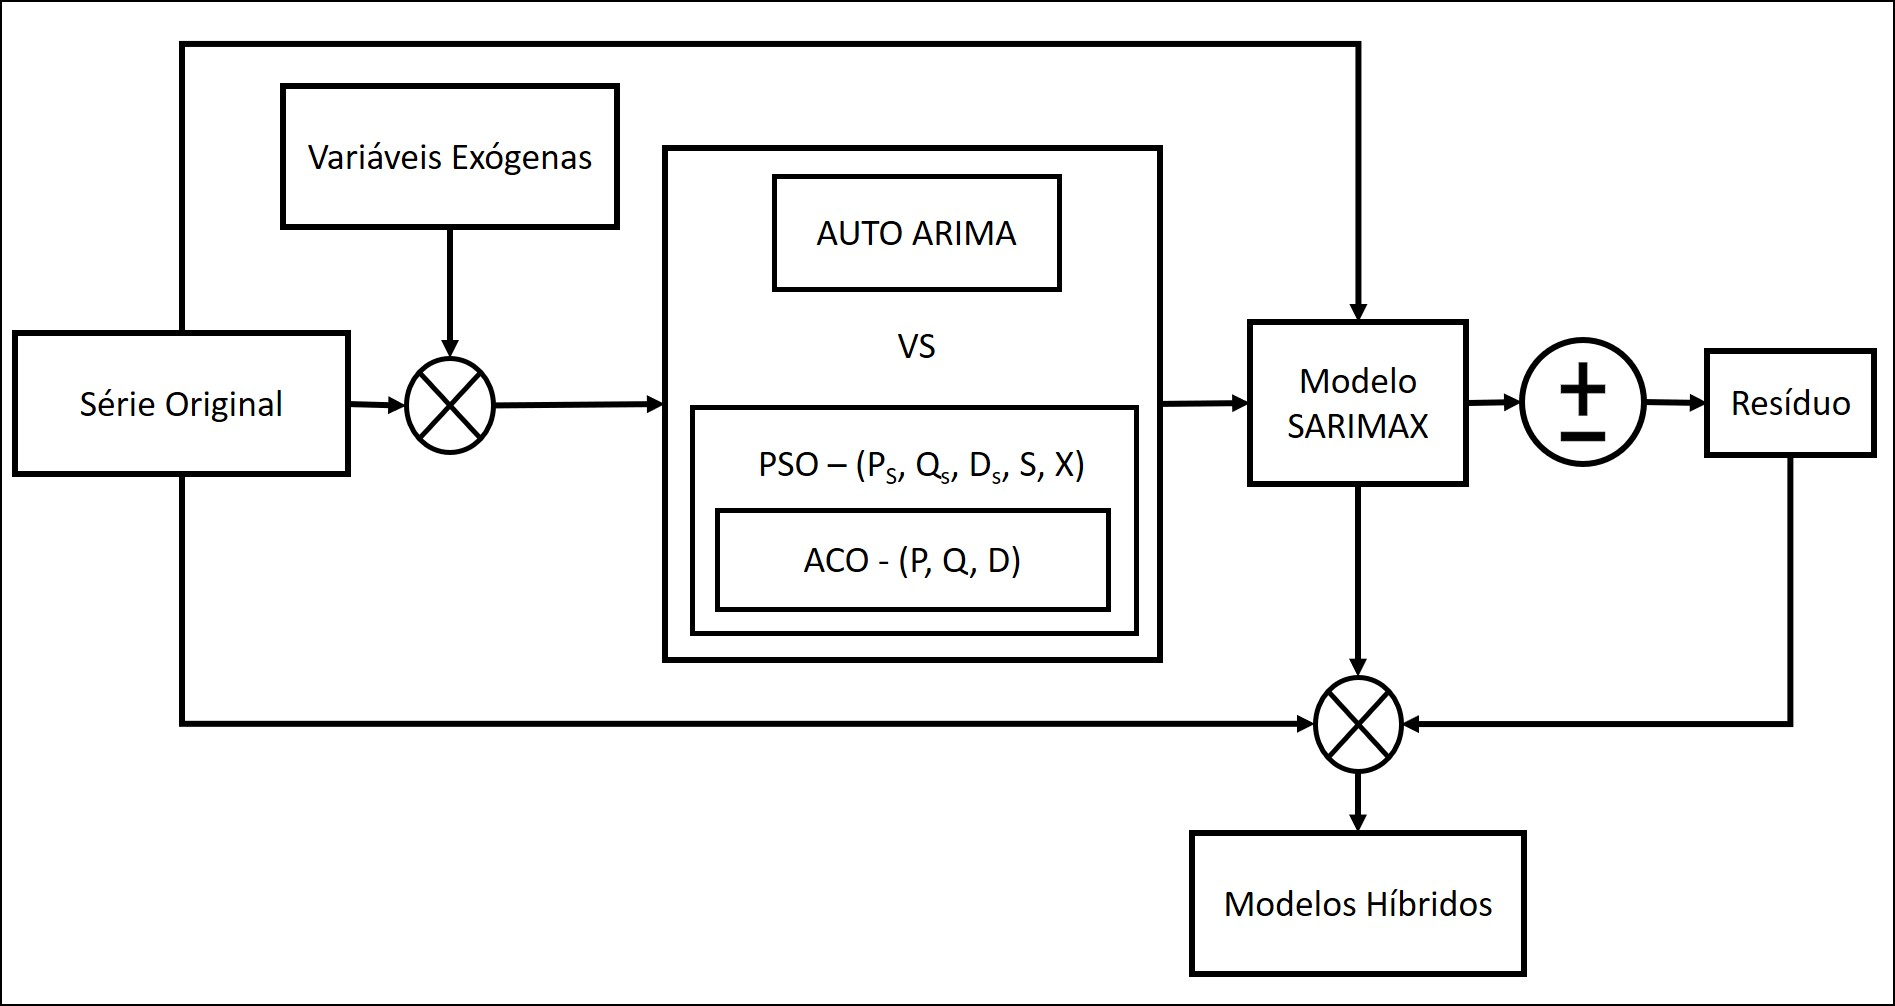
\includegraphics[width=\textwidth]{Figuras/mat_e_met/fluxograma_sarimax.jpg}
    \source{Autor.}
    \label{fig:cap3_fluxograma_sarimax}
\end{figure}

\section{Modelos Híbridos por Correção de Resíduo}
\label{subsec:modelos_hibridos}

Nesta seção será explicada a forma geral de correção do resíduo, dado pelo erro entre a série temporal original e o modelo linear SARIMAX. A correção se dá a partir do fluxograma da Figura \ref{fig:cap3_fluxograma_cromossomo}. O modelo linear SARIMAX se trata da primeira etapa do processo.

\begin{figure}[htbp]
    \centering
    \caption{Fluxograma esquemático dos modelos de correção de resíduo propostos. Os cromossomos são C1-C4. Dois modelos são gerados, um para o resíduo outro para combinar o resíduo modelado com a previsão SARIMAX.}
    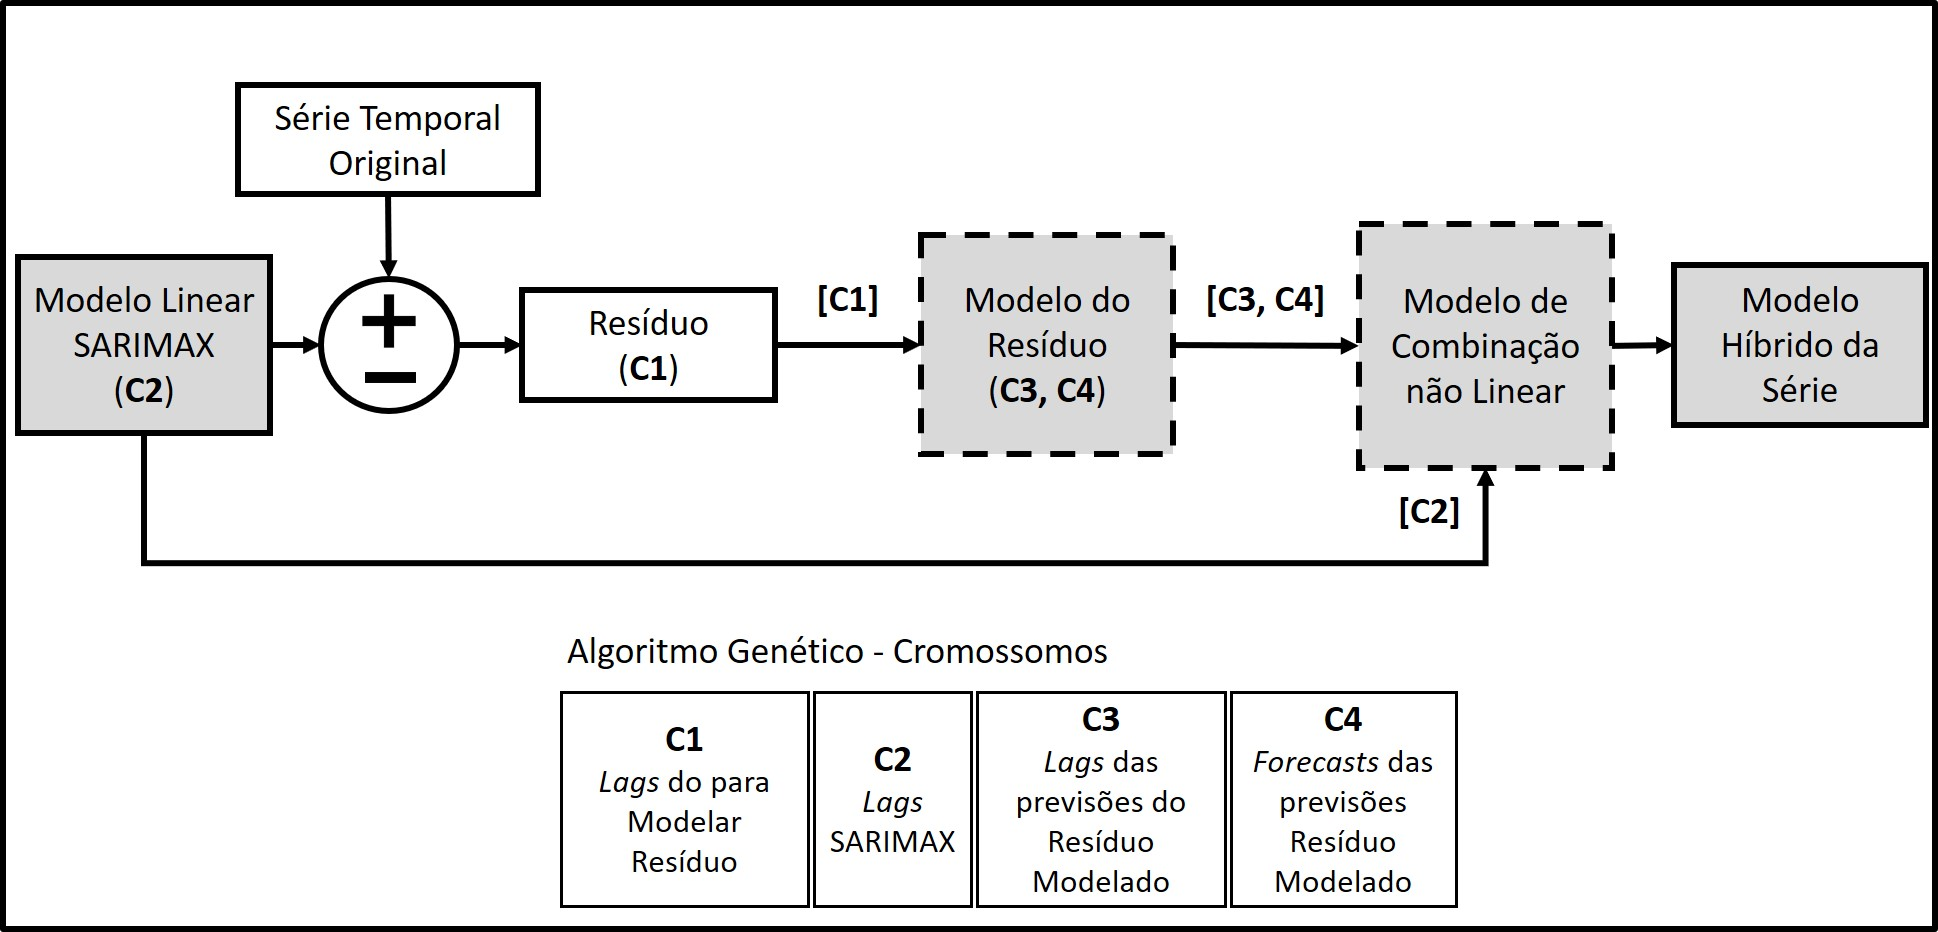
\includegraphics[width=\textwidth]{Figuras/mat_e_met/fluxograma_cromossomos.jpg}
    \source{Autor.}
    \label{fig:cap3_fluxograma_cromossomo}
\end{figure}

Como pode ser visto, existem 4 cromossomos que são utilizados na busca por algoritmo genético. As variáveis do tipo \textit{Lags} se tratam de quantidades de amostrados do passado utilizadas para prever o futuro. Cada um dos cromossomos será melhor explicado abaixo:

\begin{itemize}
    \item C1: \textit{Lags} para Modelar Resíduo - De posse do resíduo, estas amostras são utilizadas no Modelo do Resíduo, que se trata de um objeto que também é obtido a partir de busca com algoritmo genético.
    
    \item C2: \textit{Lags} SARIMAX - De posse do Modelo Linear SARIMAX é possível obter amostras do passado da série temporal gerada por estes. Essas amostras serão utilizadas na Combinação com Amostras C3 e C4 do Resíduo Modelado.
    
    \item C3: \textit{Lags} das previsões do Resíduo Modelado - Com um Modelo ML treinado e otimizado é possível gerar a séries temporal correspondente ao Resíduo Modelado e com testa obter amostras do passado.
    
    \item C4: \textit{Forecasts} das previsões do Resíduo Modelado - Análogo ao cromossomo C3, porém com amostras a frente no tempo.
\end{itemize}

Os cromossomos C1-C4 são inicializados como números inteiros de uma distribuição uniforme de limite inferior 1 e superior 20. Foi estipulado uma probabilidade de mutação e cruzamento de 80\%.

\begin{algorithm}[!hbp]
    \Entrada{população, Prob. Cruzamento}
    \Saida{Nova população}
    \Inicio{
    Mantém o melhor indivíduo;\\
    Ordena a população \textit{fitness} do melhor ao pior;\\
    \Para{indivíduo de ordem $I$}{
    $p$ = random(0,1);\\
    \Se{$p >$ Prob. Cruzamento}{
        $C$ = conjunto aleatório de cromossomos;\\
        população[$I$][$C$] = população[$I\slash2$][$C$]
    }
    }
    }
    \caption{Cruzamento escolhido para algoritmos híbridos propostos}
    \label{algo:cap3_cruz_hibrid}
\end{algorithm}

O operador de cruzamento funciona de acordo com o Algoritmo \ref{algo:cap3_cruz_hibrid}. Os indivíduos são colocados em ordem do melhor \textit{fitness} ao pior, então o melhor indivíduo sempre é levado para a próxima população. Em seguida, para cada um dos indivíduos restantes, é definido aleatoriamente um conjunto dos quatro cromossomos que serão recebidos de um indivíduo de melhor posição, esta que é dada pela posição do individuo simetricamente. A mutação dos cromossomos se dá a partir da variação da adição de um número inteiro obtido por uma distribuição uniforme entre -2 e 2.

Ainda sobre o processo representado pela Figura \ref{fig:cap3_fluxograma_cromossomo}, é necessário explicar exatamente como as variáveis dos cromossomos são necessárias pela modelagem, esta explicação se dá melhor na Figura \ref{fig:cap3_fluxograma_modelos_res_comb}. A segunda etapa do processo é dada pelo Modelo do Resíduo e a terceira, pelo Modelo de Combinação. Em ambas estas etapas, podem ser utilizados quaisquer algoritmos de regressão para que com base nos dados de treino, se gere estes dois modelos e com dados de teste se avalie.

\begin{figure}[!htbp]
    \centering
    \caption{Fluxograma detalhado sobre requisitos do Modelo do Resíduo e Modelo de Combinação não Linear.}
    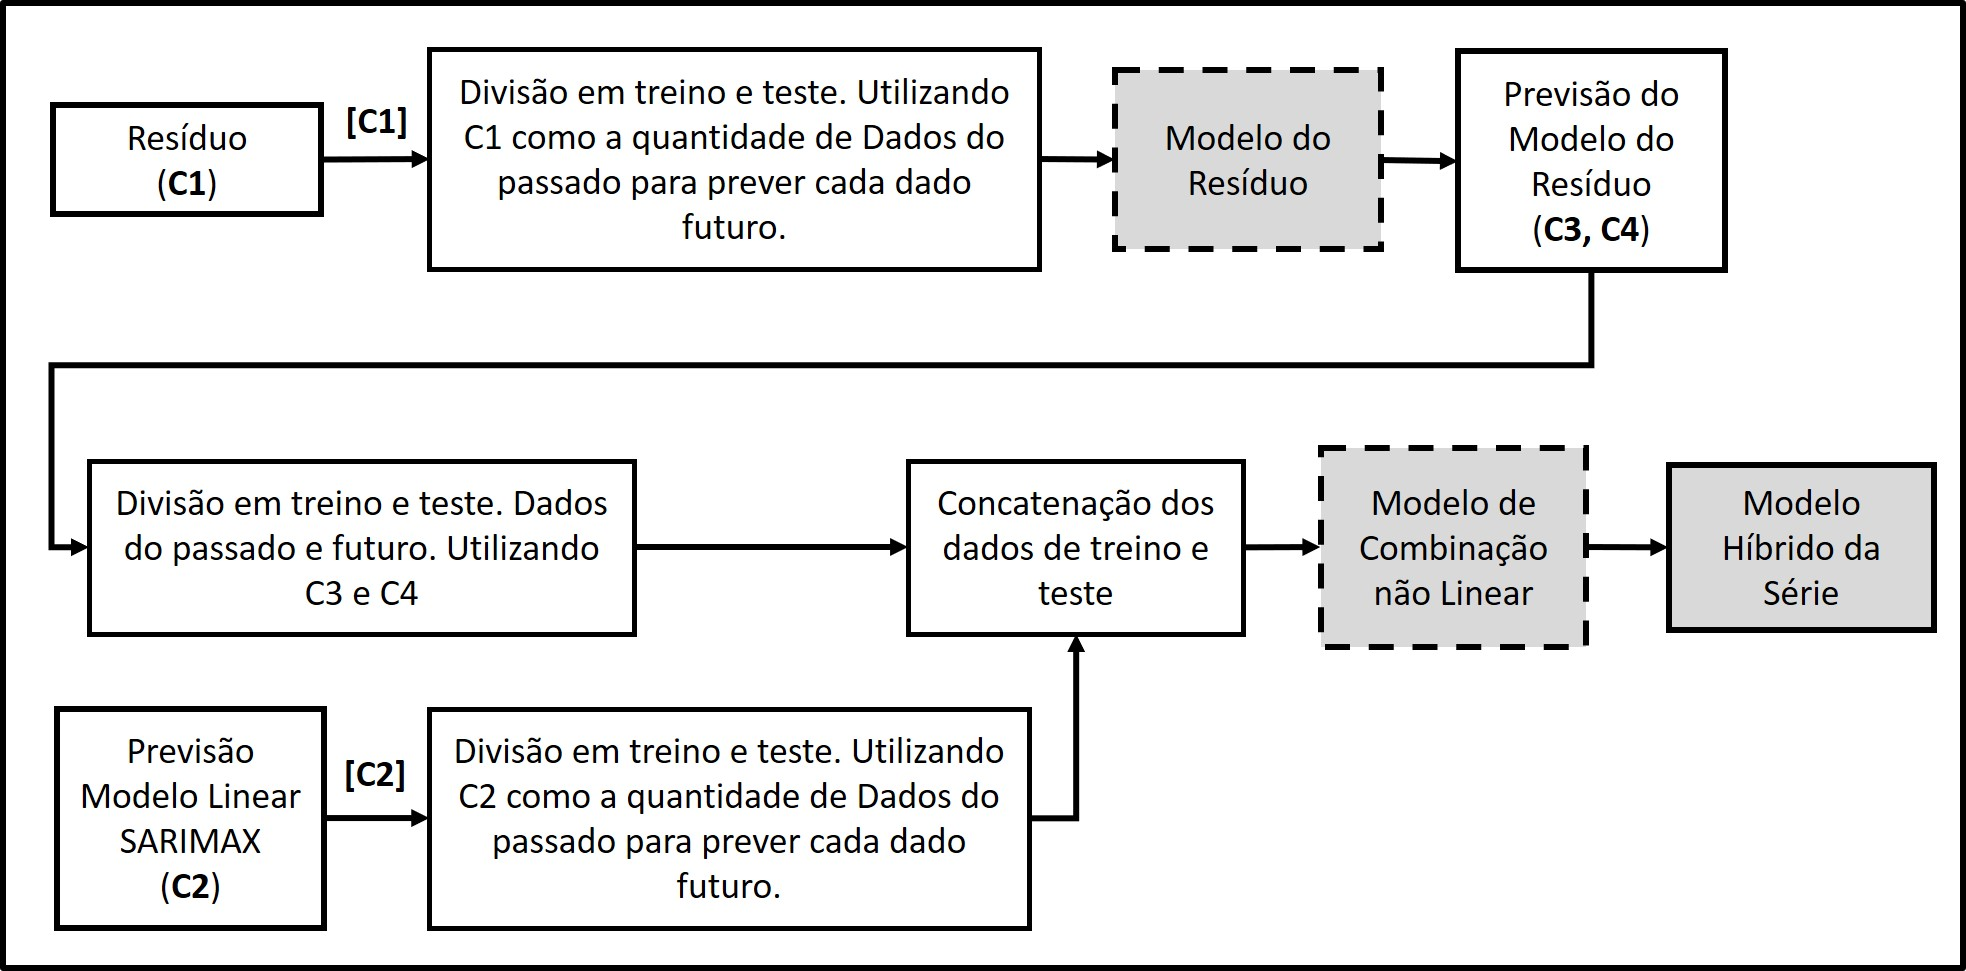
\includegraphics[width=\textwidth]{Figuras/mat_e_met/fluxograma_modelos_res_comb.jpg}
    \source{Autor.}
    \label{fig:cap3_fluxograma_modelos_res_comb}
\end{figure}

Neste trabalho para as etapas 2, Modelo do Resíduo e 3, Modelo de Combinação, podem ser escolhidos dois algoritmos de hiper-parametrização de MLPs, baseados em algoritmo genético, descritos nas próximas subseções \ref{subsec:ag-mlp} e \ref{subsec:ag-mlp-vr}.

\subsection{AG-MLP}
\label{subsec:ag-mlp}

Para obter a MLP bem parametrizada o algoritmo procura os melhores parâmetros para o MLP. Este tipo de otimização pode ser encontrado na literatura, sendo muito útil para aumentar a performance deste tipo de RNA \cite{ramchoun2016multilayer, idrissi2016genetic}. Nesta busca, o algoritmo gera uma população de MLPs, com parâmetros aleatórios, avalia estes e ranqueia o melhores parâmetros. Depois disso, uma nova população é gerada, após um cruzamento entre melhores e piores MLPs. A melhor MLP é repetida na próxima geração. Depois do cruzamento, os parâmetros numéricos sofrem mutação. Esta nova população é re-avaliada e o ciclo continua.

O algoritmo busca para cada MLP baseado nos cromossomos mostrados na Figura \ref{fig:cap3_cromo_mlp}. Para implementação das MLP é utilizada a biblioteca Scikit-learn do python \cite{scikit-learn}. É definido uma quantidade máxima de iterações em 500. Mais detalhadamente, cada um dos cromossomos tem as seguintes características:

\begin{figure}[!htbp]
    \centering
    \caption{Cromossomos do Algoritmo Genético da MLP.}
    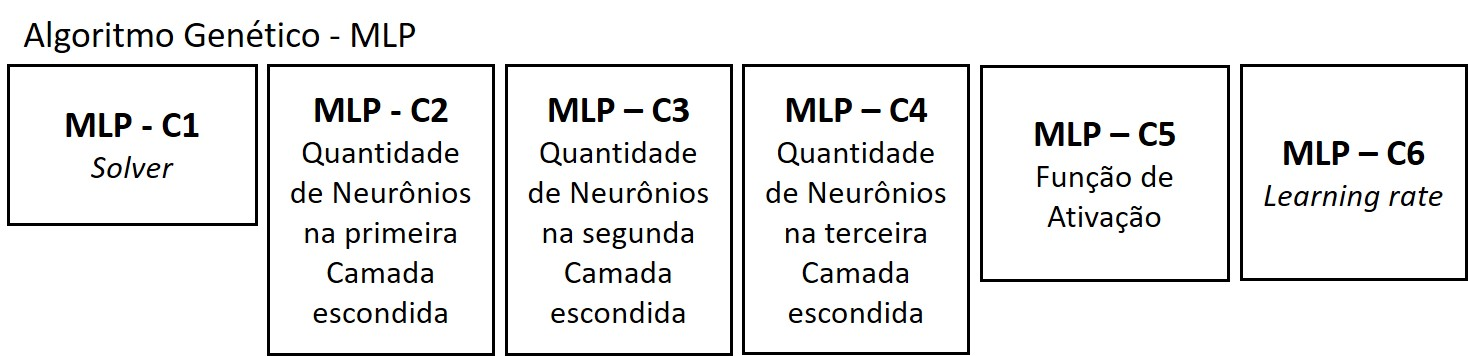
\includegraphics[width=\textwidth]{Figuras/mat_e_met/cromo_mlp.jpg}
    \source{Autor.}
    \label{fig:cap3_cromo_mlp}
\end{figure}

\begin{itemize}
    \item MLP-C1: \textit{Solver} - Se trata do algoritmo de optimização utilizado para obter os pesos nos neurônios. Pode ser escolhido entre LBFGS, ADAM e SGD. 
    
    \item MLP-C2 à MLP-C4: Quantidade de neurônios nas camada escondida 1, 2 e 3.
    
    \item MLP-C5: Função de Ativação - Possibilidade dentre as funções Identidade, Logística, Tangente Hiperbólica e Relu.
    
    \item MLP-C6: \textit{Learning Rate} - Se trata da forma que a Taxa de Aprendizagem $\eta$ da MLP é atualizada. Pode ser escolhida entre Constante, \textit{Invscaling} e Adaptativa.
    
\end{itemize}

Sobre o cromossomo \textit{Solver}, LBFGS é um acrônimo para \textit{Limited\hyp{}Memory Broyden\hyp{}Fletcher\hyp{}Goldfarb\hyp{}Shanno Algorithm} que tende a ser mais rápido que o o algoritmo SGD, acrônimo de \textit{Stochastic Gradient Descendent} \cite{le2011optimization}. No caso de uso do SGD o momento é defidno em 0.9. ADAM, cujo nome é um derivativo de \textit{Adaptative Moment Estimation}, se trata de um algoritmo cronologicamente mais novo que os anteriores e popular em aplicações envolvendo \textit{Deep Learning} \cite{kingma2014adam, yi2020effective, jais2019adam}.

Sobre o \textit{Learning Rate}, mais detalhadamente cada uma das possibilidades é caracterizada da seguinte forma: Constante é uma taxa de aprendizagem $\eta=0,001$. \textit{Invscaling} diminui gradualmente a taxa de aprendizagem periodicamente, com período $t$ usando um expoente de escala inversa como na Equação \ref{eq:learning_rate_invscaling}. A taxa de aprendizado Adaptativa mantém a taxa de aprendizagem constante enquanto a perda de treinamento continua diminuindo. Cada vez que duas épocas consecutivas falham em diminuir a perda de treinamento em pelo menos $0,0001$, ou falham em aumentar a pontuação de validação em pelo menos $0,0001$, a taxa de aprendizado atual é dividida por 5.

\begin{equation}
\label{eq:learning_rate_invscaling}
    \begin{gathered}
    \eta = \eta \slash t^{0.5}
    \end{gathered}
\end{equation}

\subsection{AG-MLP Voting Regressor}
\label{subsec:ag-mlp-vr}

Este modelo é análogo ao da Seção \ref{subsec:ag-mlp} precedente, na utilização de MLPs como elementos principais, porém com a diferença que ao invés de se escolher uma RNA apenas para o Modelo do Resíduo e Modelo de Combinação, são escolhidas as melhores RNA de forma a ser feita uma média na predição entre as melhores. Este mecanismo é chamado de \textit{Voting Regressor}. 

Para a implementação correta deste algoritmo, é adicionado um cromossomo a mais C5 aqueles que foram explicados e ilustrados na Figura \ref{fig:cap3_fluxograma_cromossomo}. 

\begin{itemize}
    \item C5: Percentagem de MLPs que farão parte do \textit{Voting Regressor}.
\end{itemize}

O cromossomo C5 tem cruzamento equivalente ao demonstrado pelo Algoritmo \ref{algo:cap3_cruz_hibrid}, porém sua mutação dá a partir da variação da adição de um número inteiro obtido por uma distribuição uniforme entre -10 e 10. 
    \chapter{Cronograma}
\label{cap:cronograma}

O desenvolvimento deste trabalho, para que todos os objetivos sejam alcançados, se dará da seguinte forma, que está sumarizada no tempo de acordo com a tabela \ref{tab:cronograma}:

\begin{enumerate}
	\item \label{crono:Atv1} Obter dados atuais de usinas fotovoltaicas por um período significativo.
	\item \label{crono:Atv2} Corrigir dados obtidos.
	\item \label{crono:Atv3} Gerar modelo linear SARIMAX com os dados obtidos.
	\item \label{crono:Atv4} Treinar modelos híbridos propostos. 
	\item \label{crono:Atv5} Avaliar modelos híbridos propostos.
	\item \label{crono:Atv6} Melhorar modelos híbridos.
	\item \label{crono:Atv7} Compilar programa de computador para aplicação dos modelos propostos. \item \label{crono:Atv8} Publicar Artigos
\end{enumerate}

\definecolor{midgray}{gray}{.3}
\begin{table}[h]
\caption{Atividades distribuídas no ano de 2021} 
\label{tab:cronograma}
\centering
	\begin{tabular}{|c|c|c|c|c|c|c|c|c|c|c|}
		\hline
		&\multicolumn{5}{c|}{2021}&\multicolumn{5}{c|}{2021}\\
		\hline
		&MAR&ABR&MAI&JUN&JUL&AGO&SET&OUT&NOV&DEZ\\
		\hline
		\ref{crono:Atv1}&\cellcolor{midgray}&\cellcolor{midgray}&&&&&&&&\\
		\hline
		\ref{crono:Atv2}&&&\cellcolor{midgray}&\cellcolor{midgray}&&&&&&\\
		\hline	
		\ref{crono:Atv3}&&&\cellcolor{midgray}&\cellcolor{midgray}&&&&&&\\
		\hline			
		\ref{crono:Atv4}&&&&\cellcolor{midgray}&\cellcolor{midgray}&&&&&\\
		\hline	
		\ref{crono:Atv5}&&&&\cellcolor{midgray}&\cellcolor{midgray}&&&&&\\
		\hline
		\ref{crono:Atv6}&&&&&\cellcolor{midgray}&\cellcolor{midgray}&&&&\\
		\hline	
		\ref{crono:Atv7}&&&&&&&\cellcolor{midgray}&\cellcolor{midgray}&&\\
		\hline
		\ref{crono:Atv8}&&&&&&&&&\cellcolor{midgray}&\cellcolor{midgray}\\
		\hline
	\end{tabular}
\end{table}
    \chapter{Resultados}
\label{cap:resultados}

\section{Resultados Esperados}
\label{sec:protocolo_resultados}

Para obtenção dos resultados é estabelecido um protocolo de uso dos modelos discutidos no capítulo de Materiáis e métodos \ref{cap:materiais_e_metodos}, sumarizados a seguir:

\begin{outline}[enumerate]
    \1 É executado o algoritmo \textbf{auto ARIMA} para obtenção do modelo SARIMAX, com frequência sazonal 24 e todas as variáveis exógenas destacadas na seção \ref{subsec:orig_data} fazendo parte da regressão.
    \1 É executado o algoritmo PSO-ACO SARIMAX.
        \2 Tendo como limite máximo de dimensionalidade para os parâmetros (p,d,q) e (P, D, Q) uma unidade acima do encontrado pelo modelo resultante do \textbf{auto ARIMA}.
        \2 A Sazonalidade é com frequência entre 24 e 48.
        \2 As variáveis exógenas são testadas para saber quais destas de fato ajudam o modelo.
            \3 Precipitação Total (mm)
            \3 Temperatura do Ar (\textdegree{}C)
            \3 Umidade Relativa (\%)
            \3 Velocidade do Vento (m/s)
            \3 Velocidade do Vento em rajada (m/s)
        \2 Se o resultado for pior que o obtido pelo \textbf{auto ARIMA}, este último é mantido. A comparação é feita a partir da métrica AICc.
    \1 O modelo SARIMAX selecionado segue para uso nos modelos híbridos descritos nas subseções \ref{subsec:ag-mlp} e \ref{subsec:ag-mlp-vr}.
        \2 Para todas as séries foi estipulado 80\% de dados para treino, que são utilizados para realizar o treinamento do algoritmo de otimização e hibridização, bem como todas as MLPs e 20\% para teste, que utilizado para avaliação do modelo híbrido final.
\end{outline}

Com base neste protocolo de uso do algoritmos propostos, nas próximas seções são apresentados resultados parciais para algumas cidades brasileiras escolhidas. Espera-se que os resultados finais sigam o mesmo padrão observado nos parciais, porém para mais localidades.

\section{Resultados Parciais}

\subsection{Maceió}

Maceió - AL é a cidade escolhida para primeiro resultado preliminar do protocolo definido. O conjunto de dados para esta cidade, se trata de 30 dias, entre 12/03/2020 às 21 horas e 11/04/2020 às 20 horas da base para a cidade de Maceió-AL. Esta localidade foi escolhida por conta da proposta do projeto de pesquisa e desenvolvimento realizado para a CHESF, também sendo importante destino turístico regional, destacando-se o "turismo de sol e mar" \cite{vasconcelos2019turismo}. A Tabela \ref{tab:cap4_comp_maceio_autoarima_psoaco} mostra o resultado da comparação entre os algoritmos descritos na seção \ref{subsec:autoarima_psoaco}. 

\begin{table}[htbp]
\caption{Comparação resultados entre \textbf{auto ARIMA} e PSO-ACO.}
\begin{center}
\begin{tabular}{ccccc}
                    & \Longstack{SARIMAX \\ (p,d,q)(P,D,Q,S)} & Variáveis Exógenas & AICc & MAPE  \\\hline
auto ARIMA & (1,0,2)(1,0,2,24) & Todas & -1488.858 & \textbf{5.3497} \\\hline
PSO-ACO             & (2,0,0)(1,0,1,24) & Temperatura do Ar & \textbf{-1516.263} & 6.7475 \\\hline
\label{tab:cap4_comp_maceio_autoarima_psoaco}
\end{tabular}
\end{center}
\end{table}

Como descrito no início do capítulo, e pelo que foi obtido, optou-se por utilizar a modelagem SARIMAX obtida descrita na segunda linha da Tabela \ref{tab:cap4_comp_maceio_autoarima_psoaco}, como entrada para os algoritmos híbridos descritos pela seções \ref{subsec:ag-mlp} e \ref{subsec:ag-mlp-vr}, resultando finalmente nos resultados descritos pela Tabela \ref{tab:cap4_comp_maceio_agmlp_agmlpvr}.Para ambos os algoritmos foram utilizadas 3 gerações e 12 indivíduos.

\begin{table}[htbp]
\caption{Comparação entre modelos para aos dados da cidade de Maceió-AL}
\begin{center}
\begin{tabular}{ccccc}
                & MAE & MSE & MAPE \\\hline
SARIMAX         & 0.035221 & 0.002941 & 2.91303 \\\hline
Híbrido AG-MLP  & \textbf{0.024321} & \textbf{0.001857} & 0.90901 \\\hline
Híbrido AG-MLP-VR & 0.02684 & 0.002439 & \textbf{0.530453} \\\hline
\label{tab:cap4_comp_maceio_agmlp_agmlpvr}
\end{tabular}
\end{center}
\end{table}

Um resultado gráfico para a localidade definida pode ser observado na Figura \ref{fig:cap4_maceio_3_days_hibrids} em que se mostra as 3 formas de modelagem e o seu resultado sobre as últimas 72 horas de dados.

\begin{figure}[!htbp]
    \centering
    \caption{Últimas 72 horas do resultado utilizando algoritmos AG-MLP e AG-MLP-VR, SARIMAX e série real. Para a cidade de Maceió-AL}
    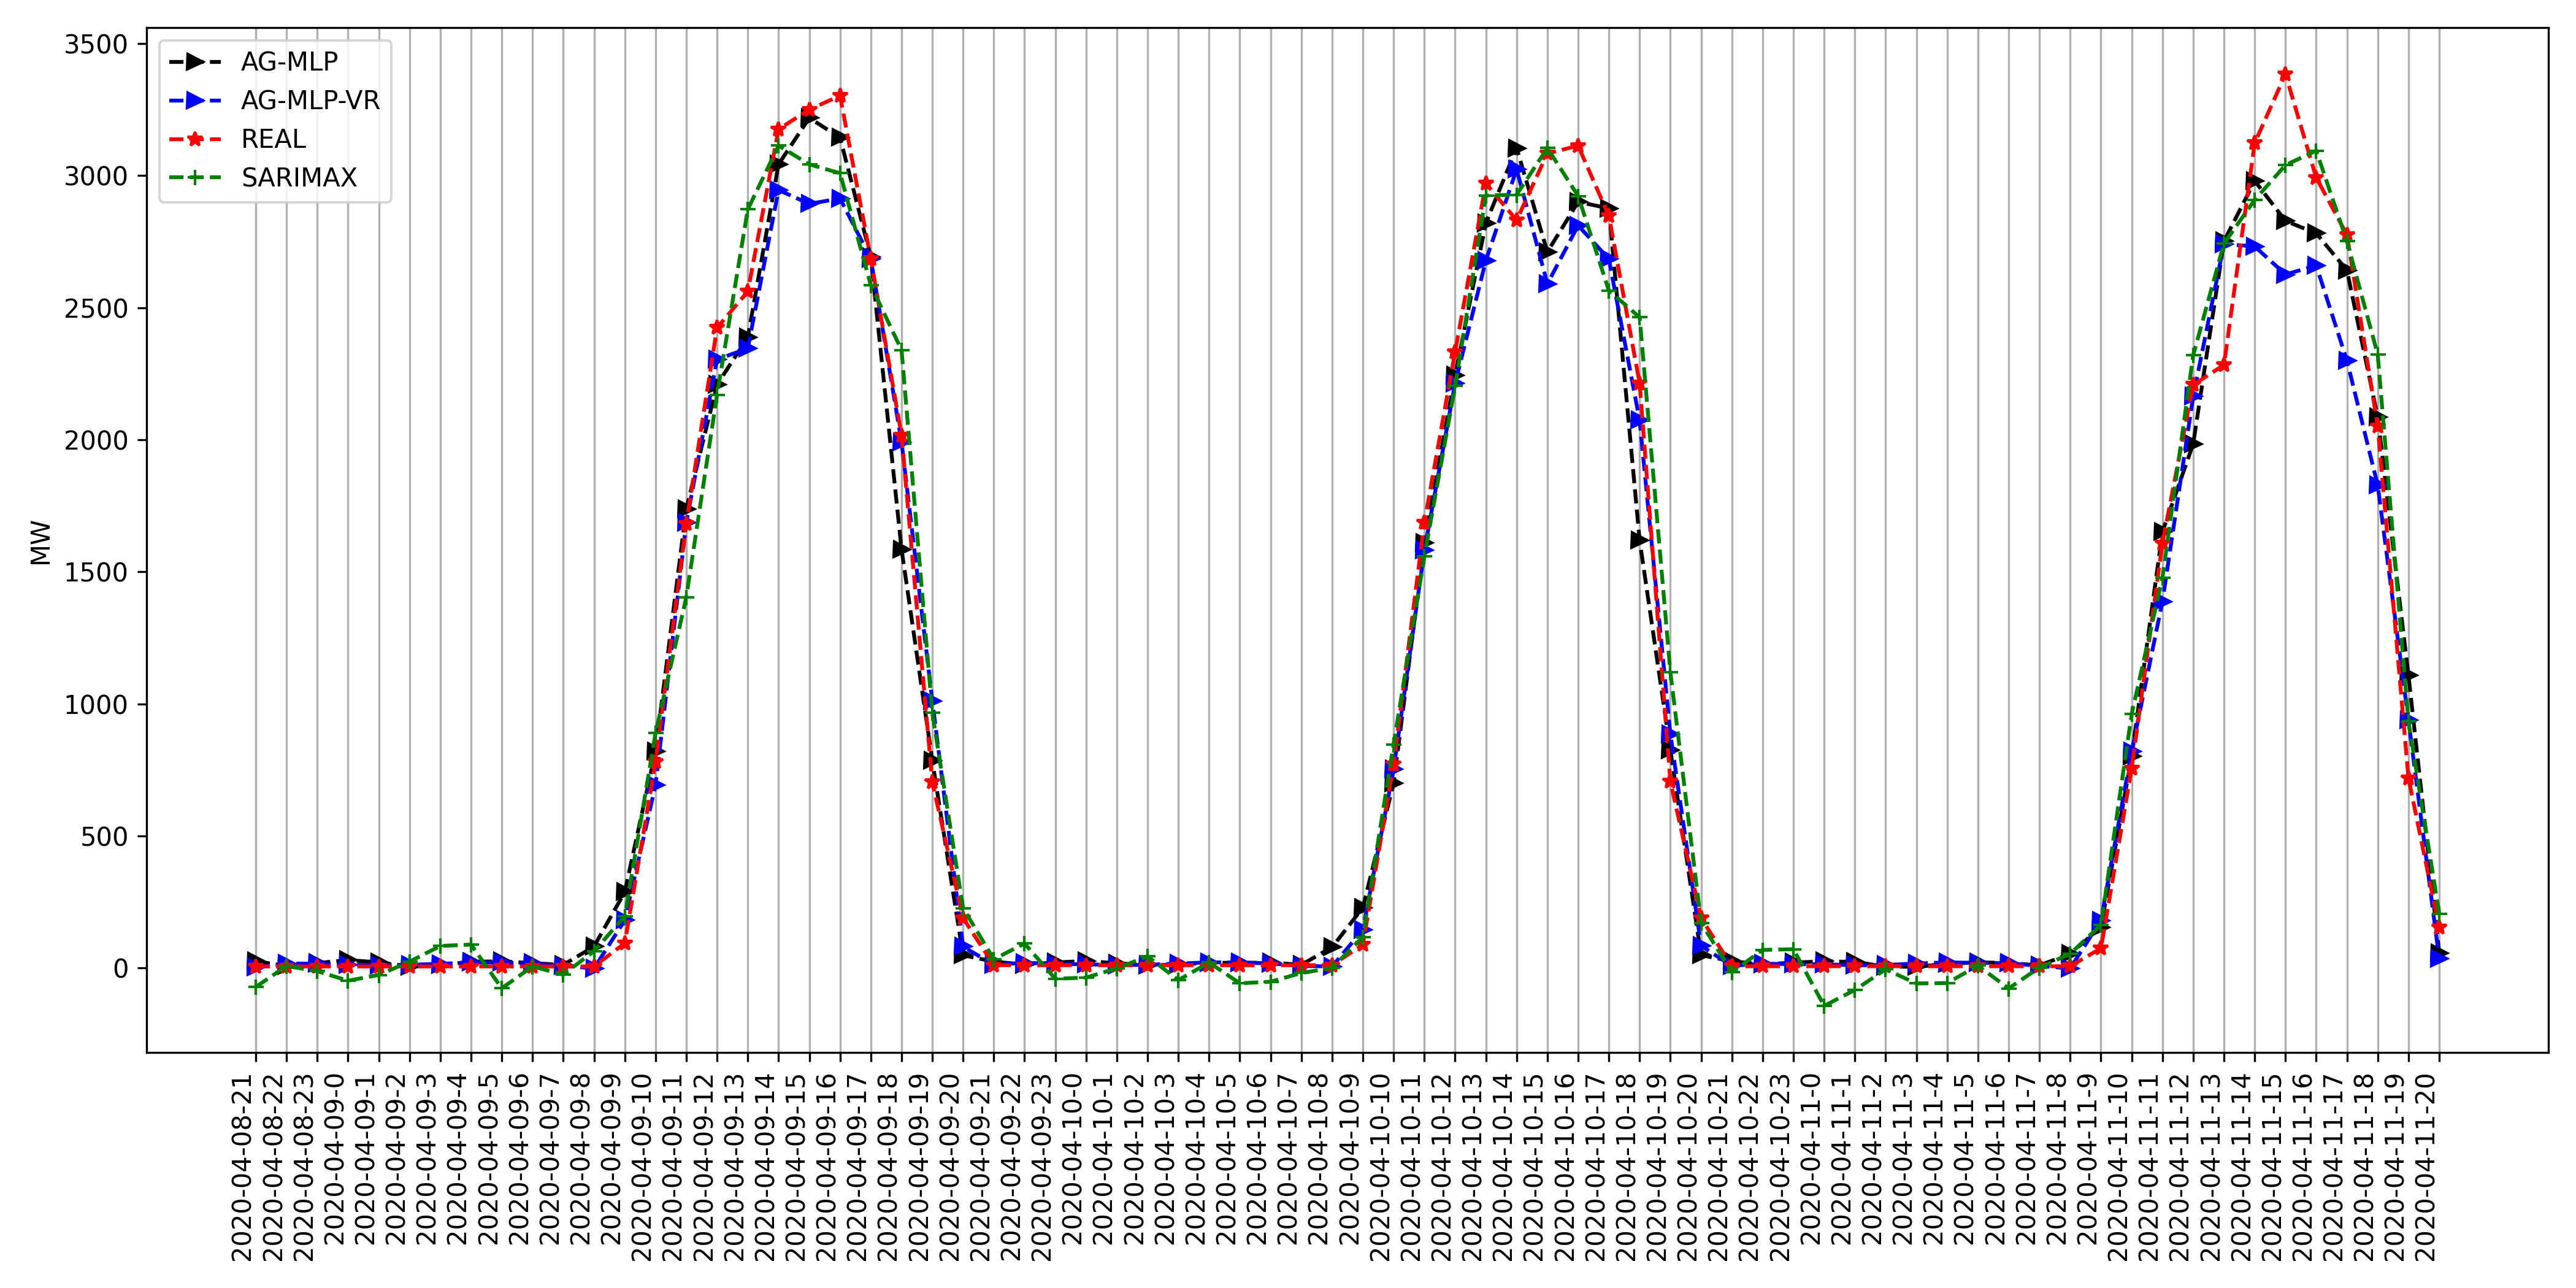
\includegraphics[width=\textwidth]{Figuras/results/comparison_hibrids_mc.png}
    \source{Autor.}
    \label{fig:cap4_maceio_3_days_hibrids}
\end{figure}

\subsection{Florianópolis}

Tendo uma região metropolitana importante economicamente, com atrativos ecoturísticos, Florianópolis-SC, foi escolhida para integrar os resultados \cite{bittencourt2015ecoturismo, cavanus2021sapiens}. Se tratando da segunda série temporal que será apresentada nos resultados deste trabalho.

São utilizados os últimos 15 dias da base obtida, entre 17/12/2019 às 0 horas e 31/12/2019 às 23 horas. A Tabela \ref{tab:cap4_comp_flor_autoarima_psoaco} mostra o resultado da comparação entre os algoritmos descritos na seção \ref{subsec:autoarima_psoaco}.

\begin{table}[htbp]
\caption{Comparação resultados entre \textbf{auto ARIMA} e PSO-ACO.}
\begin{center}
\begin{tabular}{ccccc}
                    & \Longstack{SARIMAX \\ (p,d,q)(P,D,Q,S)} & Variáveis Exógenas & AICc & MAPE  \\\hline
auto ARIMA & (0,1,1)(2,0,2,24) & Todas & -695.210 & \textbf{57.106} \\\hline
PSO-ACO             & (2,0,2)(1,0,1,24) & \Longstack{Temperatura do Ar \\ Precipitação} & \textbf{-754.4754} & 52.316 \\\hline
\label{tab:cap4_comp_flor_autoarima_psoaco}
\end{tabular}
\end{center}
\end{table}

Como descrito no início do capítulo, e pelo que foi obtido, optou-se por utilizar a modelagem SARIMAX obtida descrita na segunda linha da Tabela \ref{tab:cap4_comp_flor_autoarima_psoaco}, como entrada para os algoritmos híbridos descritos pela seções \ref{subsec:ag-mlp} e \ref{subsec:ag-mlp-vr}, resultando finalmente nos resultados descritos pela Tabela \ref{tab:cap4_comp_flor_agmlp_agmlpvr}.Para ambos os algoritmos foram utilizadas 3 gerações e 12 indivíduos.

\begin{table}[htbp]
\caption{Comparação entre modelos para aos dados da cidade de Florianópolis-SC}
\begin{center}
\begin{tabular}{ccccc}
                & MAE & MSE & MAPE \\\hline
SARIMAX         & 0.03370 & 0.00278 & 7.6349 \\\hline
Híbrido AG-MLP  & \textbf{0.01665} & \textbf{0.000818} & 1.90307 \\\hline
Híbrido AG-MLP-VR & 0.023722 & 0.00240 & \textbf{0.93862} \\\hline
\label{tab:cap4_comp_flor_agmlp_agmlpvr}
\end{tabular}
\end{center}
\end{table}

Novamente, é apresentado um resultado gráfico na Figura \ref{fig:cap4_flor_3_days_hibrids} em que se mostra as 3 formas de modelagem e o seu resultado sobre as últimas 72 horas de dados.

\begin{figure}[!htbp]
    \centering
    \caption{Últimas 72 horas do resultado utilizando algoritmos AG-MLP e AG-MLP-VR, SARIMAX e série real. Para a cidade de Florianópolis-SC}
    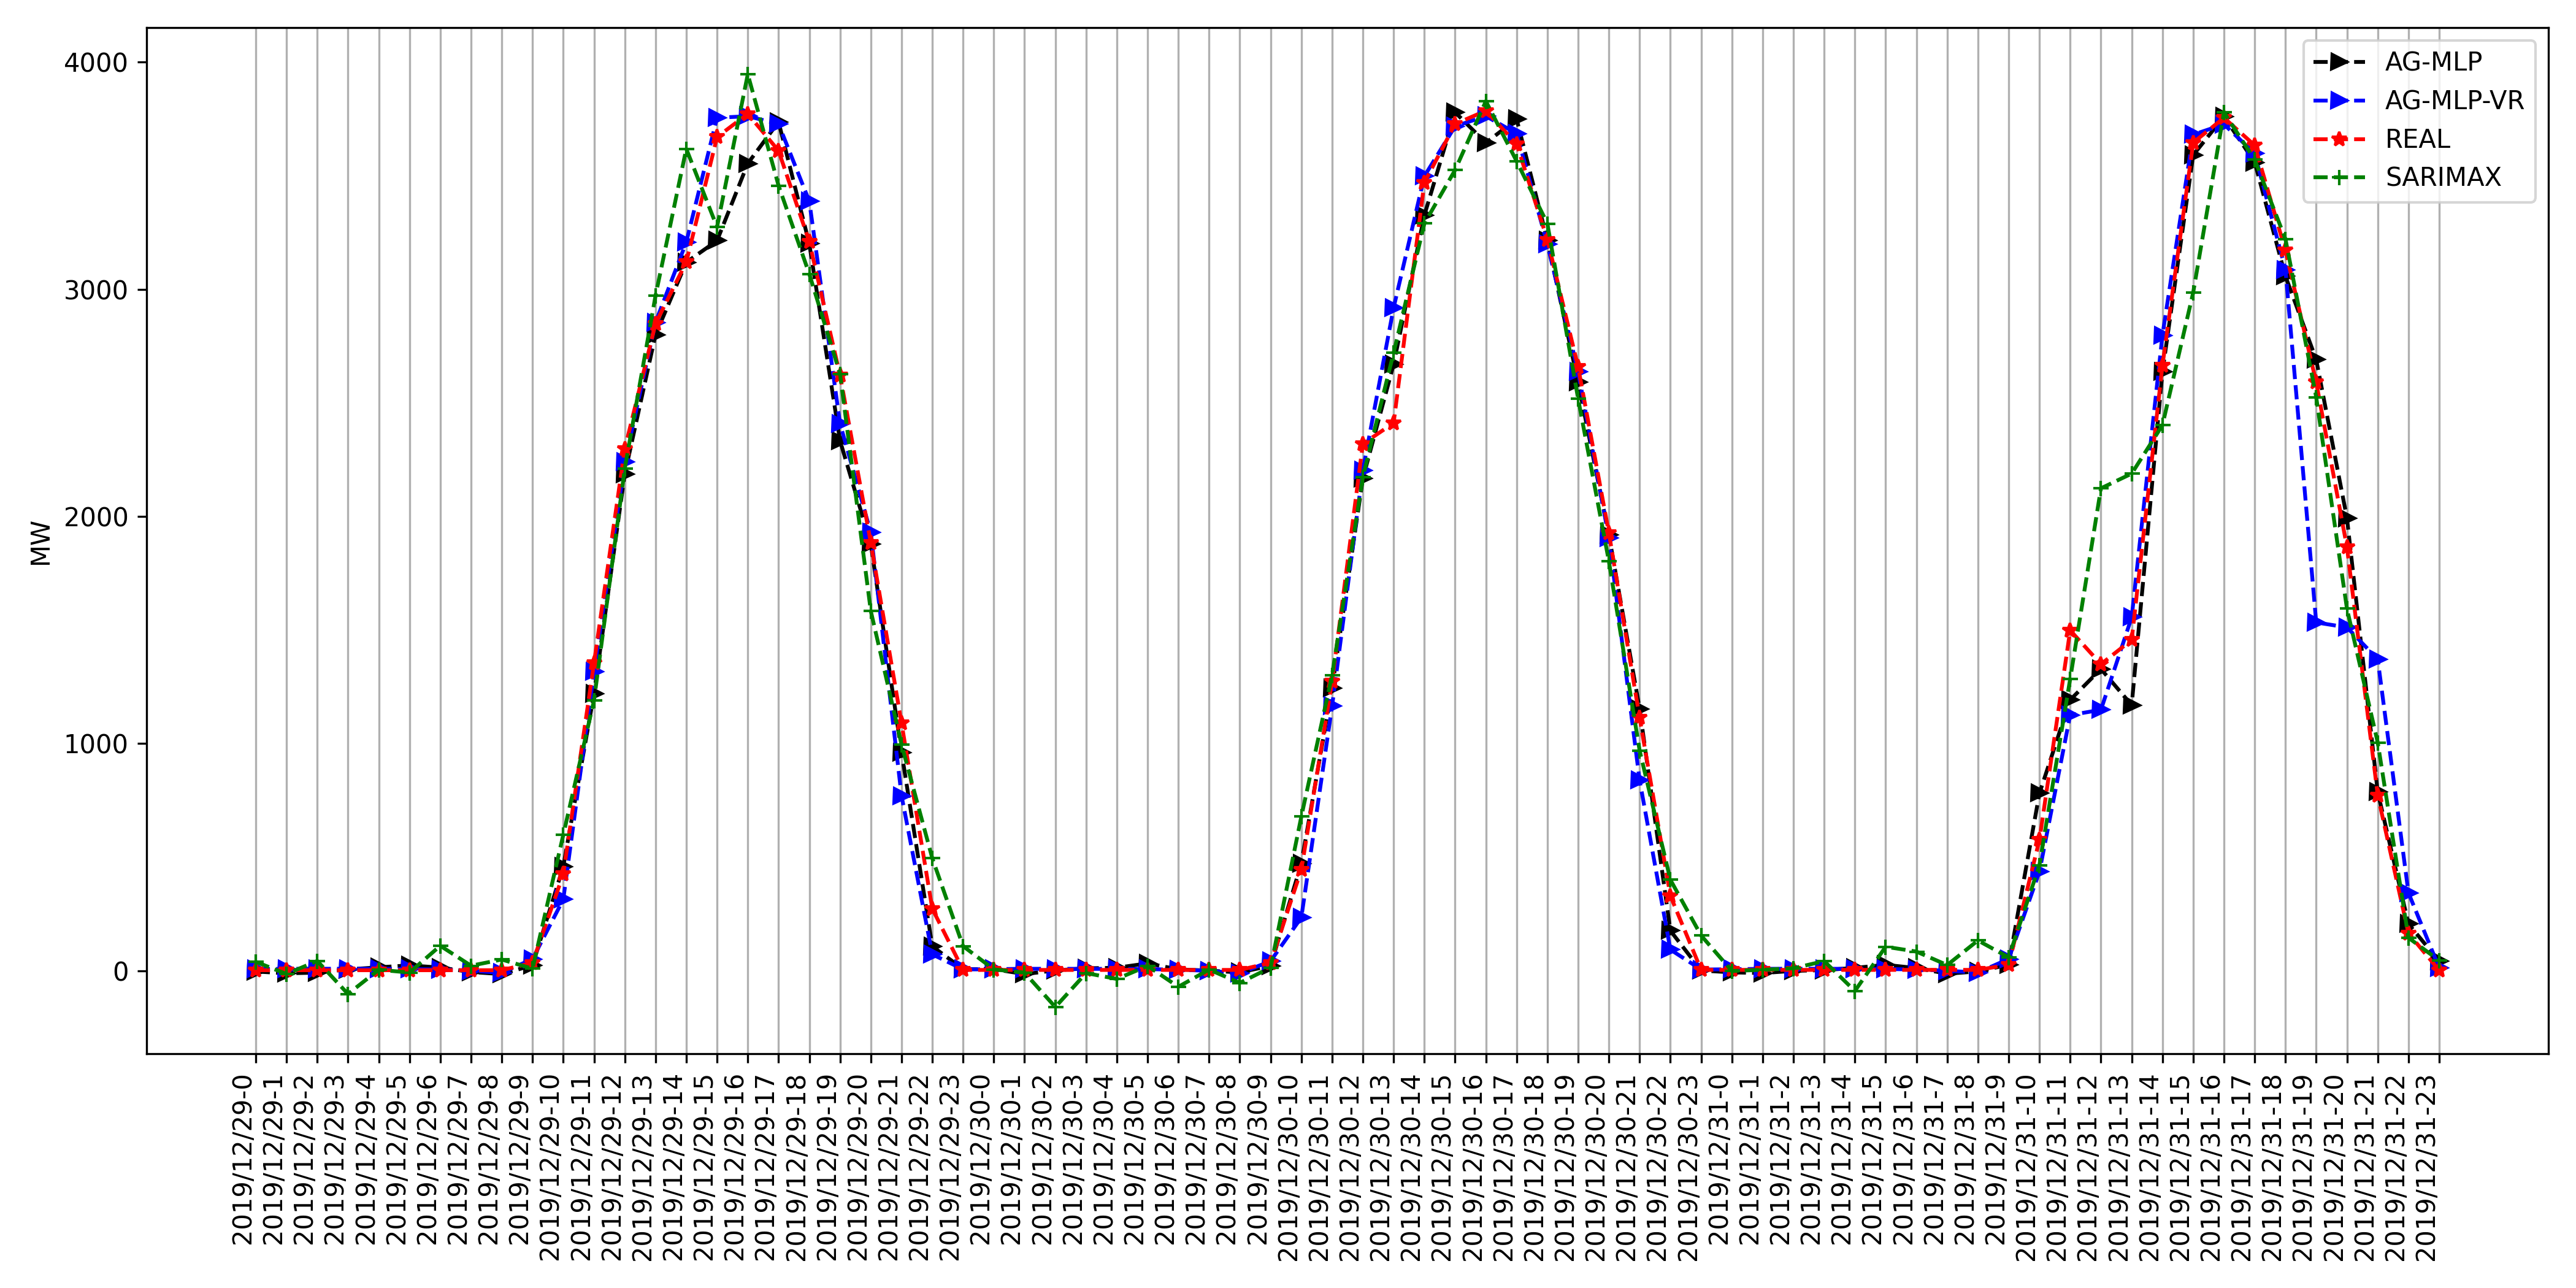
\includegraphics[width=\textwidth]{Figuras/results/comparison_hibrids_fl.png}
    \source{Autor.}
    \label{fig:cap4_flor_3_days_hibrids}
\end{figure}

\subsection{Bom Jesus da Lapa}

A terceira série temporal escolhida se trata de 15 dias, entre 17/07/2020 às 0 horas e 31/07/2020 às 23 horas da base para a cidade de Bom Jesus da Lapa - BA. Esta localidade foi escolhida por conter plantas fotovoltaicas próximas e ser um dos pontos de maior incidência de radiação fotovoltaica de acordo com o Atlas solarimétrico brasileiro \cite{pereira2017atlas}. A Tabela \ref{tab:cap4_comp_bjl_autoarima_psoaco} mostra o resultado da comparação entre os algoritmos descritos na seção \ref{subsec:autoarima_psoaco}.

\begin{table}[htbp]
\caption{Comparação resultados entre \textbf{auto ARIMA} e PSO-ACO.}
\begin{center}
\begin{tabular}{ccccc}
                    & \Longstack{SARIMAX \\ (p,d,q)(P,D,Q,S)} & Variáveis Exógenas & AICc & MAPE  \\\hline
auto ARIMA & (3,0,2)(2,0,2,24) & Todas & -825.1507 & 0.9518 \\\hline
PSO-ACO             & (1,0,0)(2,0,2,24) & \Longstack{Temperatura do Ar \\ Umidade Relativa \\ Velocidade do Vento} & \textbf{-831.802} & \textbf{0.9233} \\\hline
\label{tab:cap4_comp_bjl_autoarima_psoaco}
\end{tabular}
\end{center}
\end{table}

Como descrito no início do capítulo, e pelo que foi obtido, optou-se por utilizar a modelagem SARIMAX obtida descrita na segunda linha da Tabela \ref{tab:cap4_comp_bjl_autoarima_psoaco}, como entrada para os algoritmos híbridos descritos pela seções \ref{subsec:ag-mlp} e \ref{subsec:ag-mlp-vr}, resultando finalmente nos resultados descritos pela Tabela \ref{tab:cap4_comp_bjl_agmlp_agmlpvr}. Para ambos os algoritmos foram utilizadas 4 gerações e 15 indivíduos.

\begin{table}[htbp]
\caption{Comparação entre modelos para aos dados da cidade de Florianópolis-SC}
\begin{center}
\begin{tabular}{ccccc}
                & MAE & MSE & MAPE \\\hline
SARIMAX         & 0.03115 & \textbf{0.00252} & 0.3486 \\\hline
Híbrido AG-MLP  & \textbf{0.03105} & 0.00304 & \textbf{0.19175} \\\hline
Híbrido AG-MLP-VR & 0.03224 & 0.002783 & 0.25194 \\\hline
\label{tab:cap4_comp_bjl_agmlp_agmlpvr}
\end{tabular}
\end{center}
\end{table}

Por fim, pode ser visto na Figura \ref{fig:cap4_bjl_3_days_hibrids} um exemplo da diferença entre as séries, em que se mostra as 3 formas de modelagem e o seu resultado sobre as últimas 72 horas de dados.

\begin{figure}[!htbp]
    \centering
    \caption{Últimas 72 horas do resultado utilizando algoritmos AG-MLP e AG-MLP-VR, SARIMAX e série real. Para a cidade de Bom Jesus da Lapa - BA}
    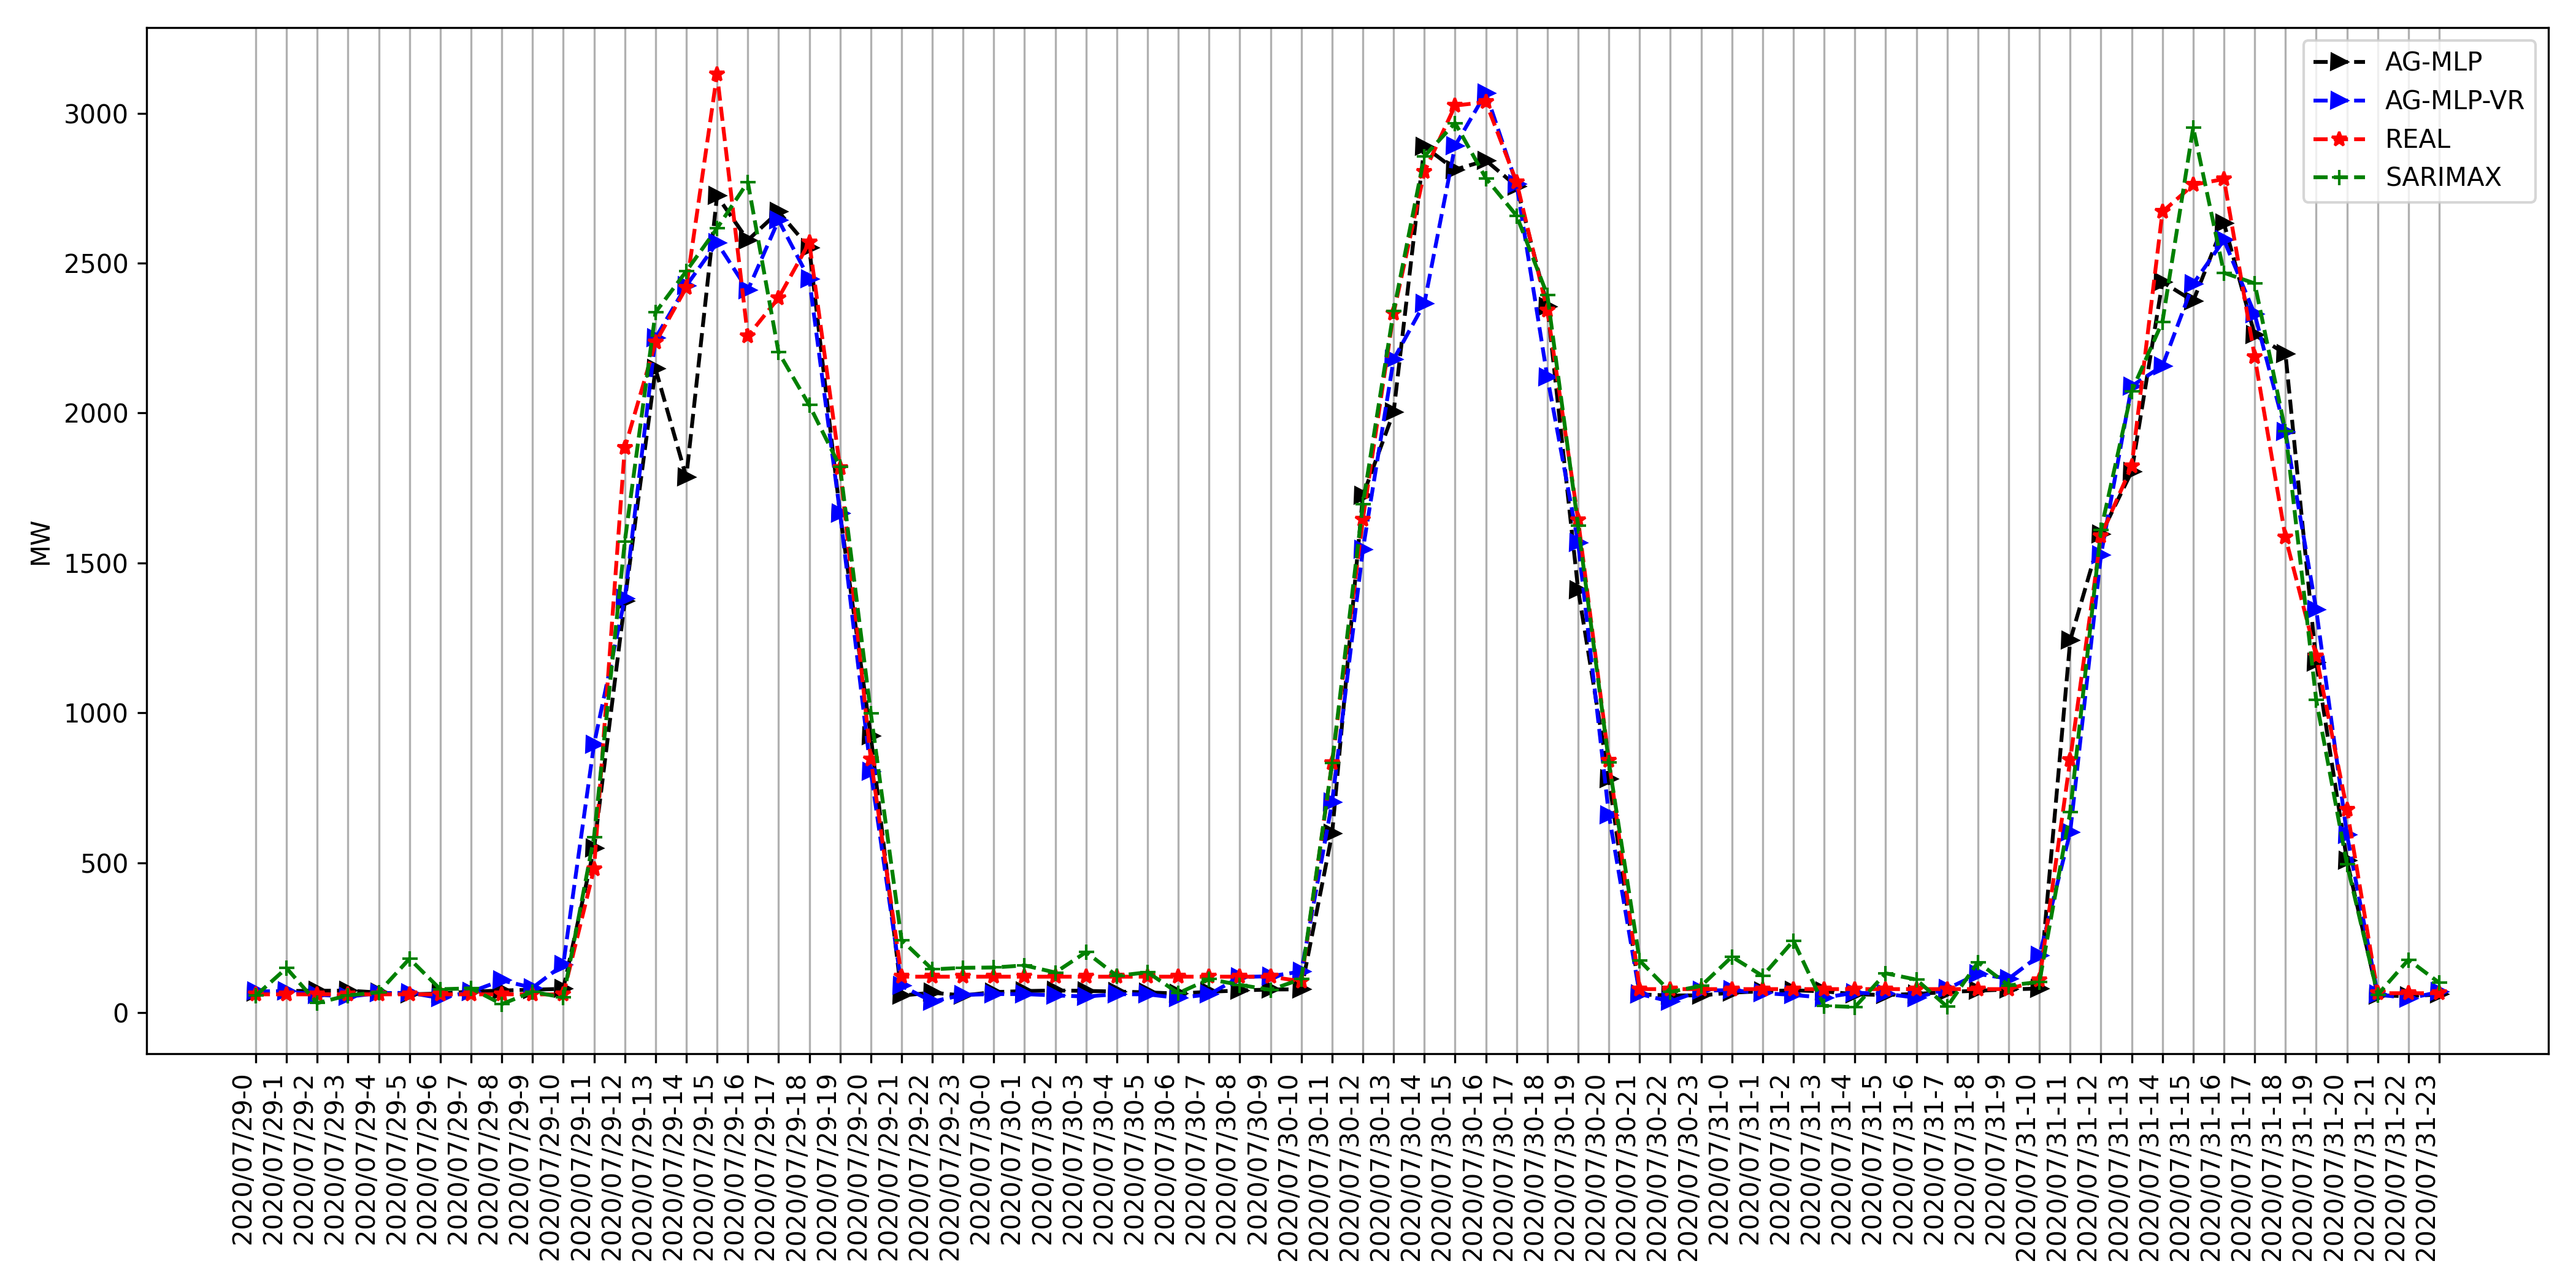
\includegraphics[width=\textwidth]{Figuras/results/comparison_hibrids_bjl.png}
    \source{Autor.}
    \label{fig:cap4_bjl_3_days_hibrids}
\end{figure}


    \chapter{Conclusões}
\label{cap:_conclusoes}

%
%%%%%%%%%%%%%%%%%%%%%%%%%%%%%%%%
%
\section{Sugestões para Trabalhos Futuros}

    
%%%%%%%%%%%%%%%%%%%%%%%%%%%%%%%%%%%%%%%%%%%%%%%%%%%%%%%%%%%%%%%%%
%                     REFERÊNCIAS UTILIZADAS                    %
%%%%%%%%%%%%%%%%%%%%%%%%%%%%%%%%%%%%%%%%%%%%%%%%%%%%%%%%%%%%%%%%%

    \addcontentsline{toc}{chapter}{\bibname}
    \bibliographystyle{abntex2-alf}
    \bibliography{Bibliografia/Bibliografia}

%%%%%%%%%%%%%%%%%%%%%%%%%%%%%%%%%%%%%%%%%%%%%%%%%%%%%%%%%%%%%%%%%
%                       APÊNDICES E ANEXOS                      %
%%%%%%%%%%%%%%%%%%%%%%%%%%%%%%%%%%%%%%%%%%%%%%%%%%%%%%%%%%%%%%%%%

	%\appendix 
\chapter{Apêndice}\label{cap:apendiceA}


\end{document} 